\documentclass[10pt,a4paper,oneside,reqno]{amsart}

\usepackage{amsmath,geometry}
\usepackage{amssymb,mathpartir,mathtools}
\usepackage{latexsym}
\usepackage{amsthm}
 \usepackage[show]{ed}
\usepackage{leftidx}
\usepackage{tikz}
\usepackage[all]{xy}
\newcommand{\xycenter}[1]{\vcenter{\hbox{\xymatrix{#1}}}}
\SelectTips{cm}{}
% Proof trees
\message{<Paul Taylor's Proof Trees, 2 August 1996>}
%% Build proof tree for Natural Deduction, Sequent Calculus, etc.
%% WITH SHORTENING OF PROOF RULES!
%% Paul Taylor, begun 10 Oct 1989
%% *** THIS IS ONLY A PRELIMINARY VERSION AND THINGS MAY CHANGE! ***
%%
%% 2 Aug 1996: fixed \mscount and \proofdotnumber
%%
%%      \prooftree
%%              hyp1            produces:
%%              hyp2
%%              hyp3            hyp1    hyp2    hyp3
%%      \justifies              -------------------- rulename
%%              concl                   concl
%%      \thickness=0.08em
%%      \shiftright 2em
%%      \using
%%              rulename
%%      \endprooftree
%%
%% where the hypotheses may be similar structures or just formulae.
%%
%% To get a vertical string of dots instead of the proof rule, do
%%
%%      \prooftree                      which produces:
%%              [hyp]
%%      \using                                  [hyp]
%%              name                              .
%%      \proofdotseparation=1.2ex                 .name
%%      \proofdotnumber=4                         .
%%      \leadsto                                  .
%%              concl                           concl
%%      \endprooftree
%%
%% Within a prooftree, \[ and \] may be used instead of \prooftree and
%% \endprooftree; this is not permitted at the outer level because it
%% conflicts with LaTeX. Also,
%%      \Justifies
%% produces a double line. In LaTeX you can use \begin{prooftree} and
%% \end{prootree} at the outer level (however this will not work for the inner
%% levels, but in any case why would you want to be so verbose?).
%%
%% All of of the keywords except \prooftree and \endprooftree are optional
%% and may appear in any order. They may also be combined in \newcommand's
%% eg "\def\Cut{\using\sf cut\thickness.08em\justifies}" with the abbreviation
%% "\prooftree hyp1 hyp2 \Cut \concl \endprooftree". This is recommended and
%% some standard abbreviations will be found at the end of this file.
%%
%% \thickness specifies the breadth of the rule in any units, although
%% font-relative units such as "ex" or "em" are preferable.
%% It may optionally be followed by "=".
%% \proofrulebreadth=.08em or \setlength\proofrulebreadth{.08em} may also be
%% used either in place of \thickness or globally; the default is 0.04em.
%% \proofdotseparation and \proofdotnumber control the size of the
%% string of dots
%%
%% If proof trees and formulae are mixed, some explicit spacing is needed,
%% but don't put anything to the left of the left-most (or the right of
%% the right-most) hypothesis, or put it in braces, because this will cause
%% the indentation to be lost.
%%
%% By default the conclusion is centered wrt the left-most and right-most
%% immediate hypotheses (not their proofs); \shiftright or \shiftleft moves
%% it relative to this position. (Not sure about this specification or how
%% it should affect spreading of proof tree.)
%
% global assignments to dimensions seem to have the effect of stretching
% diagrams horizontally.
%
%%==========================================================================

\def\introrule{{\cal I}}\def\elimrule{{\cal E}}%%
\def\andintro{\using{\land}\introrule\justifies}%%
\def\impelim{\using{\Rightarrow}\elimrule\justifies}%%
\def\allintro{\using{\forall}\introrule\justifies}%%
\def\allelim{\using{\forall}\elimrule\justifies}%%
\def\falseelim{\using{\bot}\elimrule\justifies}%%
\def\existsintro{\using{\exists}\introrule\justifies}%%

%% #1 is meant to be 1 or 2 for the first or second formula
\def\andelim#1{\using{\land}#1\elimrule\justifies}%%
\def\orintro#1{\using{\lor}#1\introrule\justifies}%%

%% #1 is meant to be a label corresponding to the discharged hypothesis/es
\def\impintro#1{\using{\Rightarrow}\introrule_{#1}\justifies}%%
\def\orelim#1{\using{\lor}\elimrule_{#1}\justifies}%%
\def\existselim#1{\using{\exists}\elimrule_{#1}\justifies}

%%==========================================================================

\newdimen\proofrulebreadth \proofrulebreadth=.05em
\newdimen\proofdotseparation \proofdotseparation=1.25ex
\newdimen\proofrulebaseline \proofrulebaseline=2ex
\newcount\proofdotnumber \proofdotnumber=3
\let\then\relax
\def\hfi{\hskip0pt plus.0001fil}
\mathchardef\squigto="3A3B
%
% flag where we are
\newif\ifinsideprooftree\insideprooftreefalse
\newif\ifonleftofproofrule\onleftofproofrulefalse
\newif\ifproofdots\proofdotsfalse
\newif\ifdoubleproof\doubleprooffalse
\let\wereinproofbit\relax
%
% dimensions and boxes of bits
\newdimen\shortenproofleft
\newdimen\shortenproofright
\newdimen\proofbelowshift
\newbox\proofabove
\newbox\proofbelow
\newbox\proofrulename
%
% miscellaneous commands for setting values
\def\shiftproofbelow{\let\next\relax\afterassignment\setshiftproofbelow\dimen0 }
\def\shiftproofbelowneg{\def\next{\multiply\dimen0 by-1 }%
\afterassignment\setshiftproofbelow\dimen0 }
\def\setshiftproofbelow{\next\proofbelowshift=\dimen0 }
\def\setproofrulebreadth{\proofrulebreadth}

%=============================================================================
\def\prooftree{% NESTED ZERO (\ifonleftofproofrule)
%
% first find out whether we're at the left-hand end of a proof rule
\ifnum  \lastpenalty=1
\then   \unpenalty
\else   \onleftofproofrulefalse
\fi
%
% some space on left (except if we're on left, and no infinity for outermost)
\ifonleftofproofrule
\else   \ifinsideprooftree
        \then   \hskip.5em plus1fil
        \fi
\fi
%
% begin our proof tree environment
\bgroup% NESTED ONE (\proofbelow, \proofrulename, \proofabove,
%               \shortenproofleft, \shortenproofright, \proofrulebreadth)
\setbox\proofbelow=\hbox{}\setbox\proofrulename=\hbox{}%
\let\justifies\proofover\let\leadsto\proofoverdots\let\Justifies\proofoverdbl
\let\using\proofusing\let\[\prooftree
\ifinsideprooftree\let\]\endprooftree\fi
\proofdotsfalse\doubleprooffalse
\let\thickness\setproofrulebreadth
\let\shiftright\shiftproofbelow \let\shift\shiftproofbelow
\let\shiftleft\shiftproofbelowneg
\let\ifwasinsideprooftree\ifinsideprooftree
\insideprooftreetrue
%
% now begin to set the top of the rule (definitions local to it)
\setbox\proofabove=\hbox\bgroup$\displaystyle % NESTED TWO
\let\wereinproofbit\prooftree
%
% these local variables will be copied out:
\shortenproofleft=0pt \shortenproofright=0pt \proofbelowshift=0pt
%
% flags to enable inner proof tree to detect if on left:
\onleftofproofruletrue\penalty1
}

%=============================================================================
% end whatever box and copy crucial values out of it
\def\eproofbit{% NESTED TWO
%
% various hacks applicable to hypothesis list 
\ifx    \wereinproofbit\prooftree
\then   \ifcase \lastpenalty
        \then   \shortenproofright=0pt  % 0: some other object, no indentation
        \or     \unpenalty\hfil         % 1: empty hypotheses, just glue
        \or     \unpenalty\unskip       % 2: just had a tree, remove glue
        \else   \shortenproofright=0pt  % eh?
        \fi
\fi
%
% pass out crucial values from scope
\global\dimen0=\shortenproofleft
\global\dimen1=\shortenproofright
\global\dimen2=\proofrulebreadth
\global\dimen3=\proofbelowshift
\global\dimen4=\proofdotseparation
\global\count255=\proofdotnumber
%
% end the box
$\egroup  % NESTED ONE
%
% restore the values
\shortenproofleft=\dimen0
\shortenproofright=\dimen1
\proofrulebreadth=\dimen2
\proofbelowshift=\dimen3
\proofdotseparation=\dimen4
\proofdotnumber=\count255
}

%=============================================================================
\def\proofover{% NESTED TWO
\eproofbit % NESTED ONE
\setbox\proofbelow=\hbox\bgroup % NESTED TWO
\let\wereinproofbit\proofover
$\displaystyle
}%
%
%=============================================================================
\def\proofoverdbl{% NESTED TWO
\eproofbit % NESTED ONE
\doubleprooftrue
\setbox\proofbelow=\hbox\bgroup % NESTED TWO
\let\wereinproofbit\proofoverdbl
$\displaystyle
}%
%
%=============================================================================
\def\proofoverdots{% NESTED TWO
\eproofbit % NESTED ONE
\proofdotstrue
\setbox\proofbelow=\hbox\bgroup % NESTED TWO
\let\wereinproofbit\proofoverdots
$\displaystyle
}%
%
%=============================================================================
\def\proofusing{% NESTED TWO
\eproofbit % NESTED ONE
\setbox\proofrulename=\hbox\bgroup % NESTED TWO
\let\wereinproofbit\proofusing
\kern0.3em$
}

%=============================================================================
\def\endprooftree{% NESTED TWO
\eproofbit % NESTED ONE
% \dimen0 =     length of proof rule
% \dimen1 =     indentation of conclusion wrt rule
% \dimen2 =     new \shortenproofleft, ie indentation of conclusion
% \dimen3 =     new \shortenproofright, ie
%                space on right of conclusion to end of tree
% \dimen4 =     space on right of conclusion below rule
  \dimen5 =0pt% spread of hypotheses
% \dimen6, \dimen7 = height & depth of rule
%
% length of rule needed by proof above
\dimen0=\wd\proofabove \advance\dimen0-\shortenproofleft
\advance\dimen0-\shortenproofright
%
% amount of spare space below
\dimen1=.5\dimen0 \advance\dimen1-.5\wd\proofbelow
\dimen4=\dimen1
\advance\dimen1\proofbelowshift \advance\dimen4-\proofbelowshift
%
% conclusion sticks out to left of immediate hypotheses
\ifdim  \dimen1<0pt
\then   \advance\shortenproofleft\dimen1
        \advance\dimen0-\dimen1
        \dimen1=0pt
%       now it sticks out to left of tree!
        \ifdim  \shortenproofleft<0pt
        \then   \setbox\proofabove=\hbox{%
                        \kern-\shortenproofleft\unhbox\proofabove}%
                \shortenproofleft=0pt
        \fi
\fi
%
% and to the right
\ifdim  \dimen4<0pt
\then   \advance\shortenproofright\dimen4
        \advance\dimen0-\dimen4
        \dimen4=0pt
\fi
%
% make sure enough space for label
\ifdim  \shortenproofright<\wd\proofrulename
\then   \shortenproofright=\wd\proofrulename
\fi
%
% calculate new indentations
\dimen2=\shortenproofleft \advance\dimen2 by\dimen1
\dimen3=\shortenproofright\advance\dimen3 by\dimen4
%
% make the rule or dots, with name attached
\ifproofdots
\then
        \dimen6=\shortenproofleft \advance\dimen6 .5\dimen0
        \setbox1=\vbox to\proofdotseparation{\vss\hbox{$\cdot$}\vss}%
        \setbox0=\hbox{%
                \advance\dimen6-.5\wd1
                \kern\dimen6
                $\vcenter to\proofdotnumber\proofdotseparation
                        {\leaders\box1\vfill}$%
                \unhbox\proofrulename}%
\else   \dimen6=\fontdimen22\the\textfont2 % height of maths axis
        \dimen7=\dimen6
        \advance\dimen6by.5\proofrulebreadth
        \advance\dimen7by-.5\proofrulebreadth
        \setbox0=\hbox{%
                \kern\shortenproofleft
                \ifdoubleproof
                \then   \hbox to\dimen0{%
                        $\mathsurround0pt\mathord=\mkern-6mu%
                        \cleaders\hbox{$\mkern-2mu=\mkern-2mu$}\hfill
                        \mkern-6mu\mathord=$}%
                \else   \vrule height\dimen6 depth-\dimen7 width\dimen0
                \fi
                \unhbox\proofrulename}%
        \ht0=\dimen6 \dp0=-\dimen7
\fi
%
% set up to centre outermost tree only
\let\doll\relax
\ifwasinsideprooftree
\then   \let\VBOX\vbox
\else   \ifmmode\else$\let\doll=$\fi
        \let\VBOX\vcenter
\fi
% this \vbox or \vcenter is the actual output:
\VBOX   {\baselineskip\proofrulebaseline \lineskip.2ex
        \expandafter\lineskiplimit\ifproofdots0ex\else-0.6ex\fi
        \hbox   spread\dimen5   {\hfi\unhbox\proofabove\hfi}%
        \hbox{\box0}%
        \hbox   {\kern\dimen2 \box\proofbelow}}\doll%
%
% pass new indentations out of scope
\global\dimen2=\dimen2
\global\dimen3=\dimen3
\egroup % NESTED ZERO
\ifonleftofproofrule
\then   \shortenproofleft=\dimen2
\fi
\shortenproofright=\dimen3
%
% some space on right and flag we've just made a tree
\onleftofproofrulefalse
\ifinsideprooftree
\then   \hskip.5em plus 1fil \penalty2
\fi
}

%==========================================================================
% IDEAS
% 1.    Specification of \shiftright and how to spread trees.
% 2.    Spacing command \m which causes 1em+1fil spacing, over-riding
%       exisiting space on sides of trees and not affecting the
%       detection of being on the left or right.
% 3.    Hack using \@currenvir to detect LaTeX environment; have to
%       use \aftergroup to pass \shortenproofleft/right out.
% 4.    (Pie in the sky) detect how much trees can be "tucked in"
% 5.    Discharged hypotheses (diagonal lines).


% Numberings 
\setcounter{tocdepth}{2}
\numberwithin{equation}{section}

% Table of contents
\makeatletter
\def\@tocline#1#2#3#4#5#6#7{\relax
\ifnum #1>\c@tocdepth % then omit
  \else 
    \par \addpenalty\@secpenalty\addvspace{#2}% 
\begingroup \hyphenpenalty\@M
    \@ifempty{#4}{%
      \@tempdima\csname r@tocindent\number#1\endcsname\relax
 }{%
   \@tempdima#4\relax
 }%
 \parindent\z@ \leftskip#3\relax \advance\leftskip\@tempdima\relax
 \rightskip\@pnumwidth plus4em \parfillskip-\@pnumwidth
 #5\leavevmode\hskip-\@tempdima #6\nobreak\relax
 \ifnum#1<0\hfill\else\dotfill\fi\hbox to\@pnumwidth{\@tocpagenum{#7}}\par
 \nobreak
 \endgroup
  \fi}
\makeatother

% Part
\makeatletter
\renewcommand{\part}{\@startsection
  {part}% name
  {0}% level
  {0mm}% indent
  {2\baselineskip}% beforeskip
  {1\baselineskip}% afterskip
  {\centering \Large\sc}}% style
\makeatother
 \renewcommand{\thepart}{\Roman{part}} 
% Section 
\makeatletter
  \renewcommand{\section}{\@startsection
  {section}% name
   {1}% level
  {0mm}% indent
   {-\baselineskip}% beforeskip
  {0.5\baselineskip}% afterskip
   {\Large\bfseries}}% style
 % Subsection  
 \renewcommand{\subsection}{\@startsection
  {subsection}% name
  {2}% level
  {0mm}% indent
  {-\baselineskip}% beforeskip
  {0.5\baselineskip}% afterskip
  {\normalfont\normalsize\bf}}% styles
\makeatother

% Theorems

\newtheoremstyle{mythm}% 
{10pt}% Space above 
{}% Space below 
{\itshape}% Body font 
{}% Indent amount 
{\bfseries}%  Theorem head font 
{.}% Punctuation after theorem head 
{.5em}% Space after theorem head 
{}% 

\newtheoremstyle{mydef}% 
{10pt}% Space above 
{3pt}% Space below 
{}% Body font 
{}% Indent amount 
{\bfseries}%  Theorem head font 
{.}% Punctuation after theorem head 
{.5em}% Space after theorem head 
{}% 

\newtheoremstyle{myrmk}% 
{10pt}% Space above 
{3pt}% Space below 
{}% Body font 
{}% Indent amount 
{\itshape}%  Theorem head font 
{.}% Punctuation after theorem head 
{.5em}% Space after theorem head 
{}% 


\theoremstyle{mythm}
\newtheorem{theorem}{Theorem}[section]
\newtheorem*{theorem*}{Theorem}
\newtheorem{lemma}[theorem]{Lemma} 
\newtheorem{proposition}[theorem]{Proposition} 
\newtheorem{corollary}[theorem]{Corollary}  
\newtheorem{apptheorem}{Theorem}
\newtheorem{atheorem}{Theorem}
\renewcommand*{\theatheorem}{\Alph{atheorem}}

\theoremstyle{mydef}
\newtheorem{definition}[theorem]{Definition}	
\newtheorem*{definition*}{Definition}	

\theoremstyle{myrmk}
\newtheorem{remark}[theorem]{Remark} 
\newtheorem{remarks}[theorem]{Remarks} 
\newtheorem*{remark*}{Remark} 
\newtheorem*{remarks*}{Remarks} 
\newtheorem{example}[theorem]{Example}
\newtheorem{examples}[theorem]{Examples}
\newtheorem*{example*}{Example}
\newtheorem*{examples*}{Examples}


% Commands
\newcommand{\ie}{\text{i.e.\ }}
\newcommand{\eg}{\text{e.g.}}
\newcommand{\resp}{\text{resp.\ }}
\newcommand{\myemph}[1]{\textit{#1}}
\newcommand{\by}[1]{\quad&&\text{by {$#1$}}}
% Definitional equality
\newcommand{\deq}{\equiv}
% Propositional equality
\newcommand{\peq}{=}
% Homotopy
\newcommand{\ho}{\sim}
% Definitions
\newcommand{\defeq}{\deq_{\mathrm{def}}}
% Colon
\newcommand{\co}{\colon}
% Composition and identiies
\newcommand{\idfun}[1]{\mathsf{id}_{#1}}
\newcommand{\comp}{\circ}
% Names for type theories
\newcommand{\Hint}{\mathcal{H}}
\newcommand{\Hext}{\mathcal{H}_{\mathrm{ext}}}
% Judgements
\newcommand{\type}{\mathsf{type}}
\newcommand{\judge}[3][]{#2\;\vdash_{#1}\;#3}
% Preliminaries
\newcommand{\isntype}[1]{\mathsf{is}\text{-}\mathsf{#1}\text{-}\mathsf{type}}
\newcommand{\iscontr}{\mathsf{iscontr}}
\newcommand{\isprop}{\mathsf{isprop}}
\newcommand{\isequiv}{\mathsf{isequiv}}
\newcommand{\hfiber}{\mathsf{hfiber}}
\newcommand{\trans}{\mathsf{tr}}
\newcommand{\ext}{\mathsf{ext}}
\renewcommand{\int}{\mathsf{int}}
\newcommand{\Hot}{\mathsf{Hot}}
\newcommand{\U}{\mathcal{U}}

\newcommand{\ct}{\cdot}
% {%
%  \mathchoice{\mathbin{\raisebox{0.5ex}{$\displaystyle\centerdot$}}}%
  %           {\mathbin{\raisebox{0.5ex}{$\centerdot$}}}%
   %         {\mathbin{\raisebox{0.25ex}{$\scriptstyle\,\centerdot\,$}}}%
     %        {\mathbin{\raisebox{0.1ex}{$\scriptscriptstyle\,\centerdot\,$}}}}
\newcommand{\funext}{\leftidx{^\Pi}{\mathsf{Eq}}^{=}}       
\newcommand{\happly}{\leftidx{^=}{\mathsf{Eq}}^{\Pi}}
\newcommand{\idtoeq}{\leftidx{^=}{\mathsf{Eq}}^{\simeq}}
\newcommand{\idtodpair}{\leftidx{^=}{\mathsf{Eq}}^{\Sigma}}
\newcommand{\canzero}{\ast_0}
\newcommand{\canone}{\ast_1}

\newcommand{\idtopair}{\mathsf{idtopair}}

% Pi-types and Sigma-types
\newcommand{\prd}[1]{\Pi_{#1}}
\newcommand{\sm}[1]{\Sigma_{#1}}    
\newcommand{\lam}[1]{\lambda_{#1}}   
\newcommand{\pair}{\mathsf{pair}}
\newcommand{\fst}{\mathsf{fst}}
\newcommand{\snd}{\mathsf{snd}}
\newcommand{\app}{\mathsf{ap}}
\newcommand{\mysplit}{\mathsf{split}}
% Empty type
\newcommand{\abort}{\mathsf{0rec}}
% List type
\newcommand{\List}{\mathsf{List}}
% Unit type
\newcommand{\Unit}{\mathsf{Unit}}
% Identity types
\newcommand{\Id}{\mathsf{Id}}
\newcommand{\id}[1]{\Id_{#1}}
\newcommand{\refl}{\mathsf{refl}}
\newcommand{\idrec}{\mathsf{J}}
% Natural numbers
\newcommand{\nat}{\ensuremath{\mathbb{N}}} 
\newcommand{\suc}{\mathsf{suc}}
% W-types
\newcommand{\W}{\mathsf{W}}
\newcommand{\wsup}{\mathsf{sup}}
\newcommand{\wrec}{\mathsf{wrec}}
\newcommand{\wind}{\mathsf{wind}}
\newcommand{\wcomp}{\mathsf{wcomp}}
\newcommand{\windcomp}{\mathsf{wind}\text{-}\mathsf{comp}}
\newcommand{\wreccomp}{\mathsf{wrec}\text{-}\mathsf{comp}}
\newcommand{\winduniq}{\mathsf{wind}\text{-}\mathsf{uniq}}
\newcommand{\wrecuniq}{\mathsf{wrec}\text{-}\mathsf{uniq}}
\newcommand{\windcoh}{\mathsf{wind}\text{-}\mathsf{coh}}
\newcommand{\wreccoh}{\mathsf{wrec}\text{-}\mathsf{coh}}
% Booleans
\newcommand{\Bool}{\mathsf{Bool}}
\newcommand{\true}{1}
\newcommand{\false}{0}
\newcommand{\one}{\mathsf{1}}
\newcommand{\zero}{\mathsf{0}}
\newcommand{\boolind}{\mathsf{ind}}
\newcommand{\boolrec}{\mathsf{rec}}
\newcommand{\boolcomp}{\mathsf{2comp}}
\newcommand{\boolindcompo}{\mathsf{2ind}\text{-}\mathsf{comp0}}
\newcommand{\boolindcompi}{\mathsf{2ind}\text{-}\mathsf{comp1}}
\newcommand{\boolinduniq}{\mathsf{2ind}\text{-}\mathsf{uniq}}
\newcommand{\boolrecuniq}{\mathsf{2rec}\text{-}\mathsf{uniq}}
\newcommand{\boolindcoho}{\mathsf{2ind}\text{-}\mathsf{coh0}}
\newcommand{\boolindcohi}{\mathsf{2ind}\text{-}\mathsf{coh1}}
\newcommand{\boolreccoho}{\mathsf{2rec}\text{-}\mathsf{coh0}}
\newcommand{\boolreccohi}{\mathsf{2rec}\text{-}\mathsf{coh1}}
\newcommand{\boolreccompo}{\mathsf{2rec}\text{-}\mathsf{comp0}}
\newcommand{\boolreccompi}{\mathsf{2rec}\text{-}\mathsf{comp1}}
% Universes
\newcommand{\UU}{\mathsf{U}}


% Bipointed types

\newcommand{\ind}{\mathsf{ind}}
\newcommand{\rec}{\mathsf{rec}}
\newcommand{\Hom}{\mathsf{Hom}}
\newcommand{\Ho}{\mathsf{Ho}}
\newcommand{\Bip}{\mathsf{Bip}}
\newcommand{\BipHom}{\mathsf{Bip}}
\newcommand{\BoolCell}{\mathsf{BipHot}}
\newcommand{\BoolFibCell}{\mathsf{BipHotSect}}
\newcommand{\HasBoolRec}{\mathsf{has}\text{-}\mathsf{2}\text{-}\mathsf{rec}}
\newcommand{\HasBoolInd}{\mathsf{has}\text{-}\mathsf{2}\text{-}\mathsf{ind}}
\newcommand{\HasBoolRecUniq}{\mathsf{has}\text{-}\mathsf{2}\text{-}\mathsf{rec}\text{-}\mathsf{uniq}}
\newcommand{\HasBoolIndUniq}{\mathsf{has}\text{-}\mathsf{2}\text{-}\mathsf{ind}\text{-}\mathsf{uniq}}
\newcommand{\FibBip}{\mathsf{FibBip}}
\newcommand{\BipSect}{\mathsf{BipSect}}
\newcommand{\ishinit}{\mathsf{ishinit}}
\newcommand{\isind}{\mathsf{isind}}
\newcommand{\BoolIdHom}{\mathsf{2}\text{-}\mathsf{Id}\text{-}\mathsf{Hom}}
\newcommand{\BoolCompHom}{\mathsf{2}\text{-}\mathsf{Comp}\text{-}\mathsf{Hom}}
\newcommand{\BipIso}{\mathsf{2}\text{-}\mathsf{Alg}\text{-}\mathsf{Iso}}
\newcommand{\isbipequiv}{\mathsf{isbipequiv}}
\newcommand{\BipEquiv}{\mathsf{BipEquiv}}
\newcommand{\BipHot}{\mathsf{BipHot}}
\newcommand{\HoSec}{\mathsf{BipHotSec}}


\newcommand{\ishinitial}{\mathsf{ishinit}}


% Successor types
\newcommand{\NatAlg}{\nat\mathsf{Alg}}
\newcommand{\NatHom}{\nat\mathsf{Hom}}
\newcommand{\HasNatRec}{\mathsf{has}\text{-}\nat\text{-}\mathsf{rec}}
\newcommand{\HasNatInd}{\mathsf{has}\text{-}\nat\text{-}\mathsf{ind}}
\newcommand{\HasNatRecUniq}{\mathsf{has}\text{-}\nat\text{-}\mathsf{rec}\text{-}\mathsf{uniq}}
\newcommand{\HasNatIndUniq}{\mathsf{has}\text{-}\nat\text{-}\mathsf{ind}\text{-}\mathsf{uniq}}
\newcommand{\NatFibAlg}{\nat\mathsf{FibAlg}}
\newcommand{\NatFibHom}{\nat\mathsf{Sect}}
\newcommand{\IsNatInit}{\mathsf{is}\text{-}\nat\text{-}\mathsf{init}}
\newcommand{\IsNatHInit}{\mathsf{is}\nat\mathsf{HomInit}}
\newcommand{\IsNatHProj}{\mathsf{is}\nat\mathsf{HomProj}}
% P-algebras
\newcommand{\Palg}{P\text{-}\mathsf{Alg}}
\newcommand{\WAlgToNatAlg}{\W\text{-}\mathsf{to}\text{-}\nat\text{-}\mathsf{Alg}}
\newcommand{\WFibAlgToNatFibAlg}{\mathsf{P}\text{-}\mathsf{to}\text{-}\nat\text{-}\mathsf{FibAlg}}
\newcommand{\WCell}{\mathsf{PHot}}
\newcommand{\WFibCell}{\mathsf{PFibHot}}
\newcommand{\WAlg}{\mathsf{PAlg}}
\newcommand{\WFibAlg}{\mathsf{PFibAlg}}
\newcommand{\WHom}{\mathsf{PHom}}
\newcommand{\WFibHom}{\mathsf{PSect}}
\newcommand{\HasWRec}{\mathsf{has}\text{-}\mathsf{W}\text{-}\mathsf{rec}}
\newcommand{\HasWInd}{\mathsf{has}\text{-}\mathsf{W}\text{-}\mathsf{ind}}
\newcommand{\HasWRecUniq}{\mathsf{has}\text{-}\mathsf{W}\text{-}\mathsf{rec}\text{-}\mathsf{uniq}}
\newcommand{\HasWIndUniq}{\mathsf{has}\text{-}\mathsf{W}\text{-}\mathsf{ind}\text{-}\mathsf{uniq}}
\newcommand{\IsWHInit}{\mathsf{isPHomInit}}
\newcommand{\IsWHProj}{\mathsf{isPHomProj}}
\newcommand{\WIdHom}{\mathsf{W}\text{-}\mathsf{Id}\text{-}\mathsf{Hom}}
\newcommand{\WCompHom}{\mathsf{W}\text{-}\mathsf{Comp}\text{-}\mathsf{Hom}}
\newcommand{\WAlgIso}{\mathsf{W}\text{-}\mathsf{Alg}\text{-}\mathsf{Eq}}
\newcommand{\wrecs}{\mathsf{rec}}
% Calligraphic letters
\newcommand{\X}{\mathcal{X}}
\newcommand{\Y}{\mathcal{Y}}
\newcommand{\Z}{\mathcal{Z}}
% Another symbol
\newcommand{\z}{\mathsf{z}}


% DOCUMENT 

\begin{document}

\title{Homotopy-initial algebras in type theory}
\author[S. Awodey]{STEVE AWODEY}
\address{Carnegie Mellon University}
\author[N. Gambino]{NICOLA GAMBINO}
\address{School of Mathematics, University of Leeds}
\author[K. Sojakova]{KRISTINA SOJAKOVA}
\address{Carnegie Mellon University}
\date{\today}



\begin{abstract}
Homotopy type theory is an interpretation of Martin-L\"of's constructive type theory into abstract homotopy theory.   There results a link between constructive mathematics and algebraic topology, providing topological semantics for intensional systems of type theory as well as a computational approach to algebraic topology via type theory-based proof assistants such as~Coq.

The present work investigates inductive types in this setting. Modified rules for inductive types, including types of well-founded trees, or W-types, are presented, and the basic homotopical semantics of such types are determined.  Proofs of all results have been formally verified by the Coq proof assistant, and the proof scripts for this verification form an essential component of this research.      
\end{abstract}


\maketitle



\begin{small}
\tableofcontents
\end{small}

%%%%%%%%%%%%%%%%%%%%%%%%%%%%%%%%%%%%%%%%%%%%%%%%%%%%%%%%%
\section{Introduction}

The general topic of Homotopy Type Theory is concerned with the study of the constructive type theories of Martin-L\"of under their new interpretation into abstract homotopy theory and higher-dimensional category theory. Martin-L\"of type theories are foundational systems which have been used to formalize large parts of constructive mathematics, and also for the development of high-level programming languages~\cite{MartinLofP:conmcp}.  They are prized for their combination of expressive strength and desirable proof-theoretic properties.  One aspect of these type theories that has led to special difficulties in providing semantics is the intensional character of equality.  In recent work \cite{AwodeyS:homtmi,VoevodskyV:notts,vandenBergB:topsmi,AwodeyS:typth}, it has emerged that the topological notion of \emph{homotopy} provides an adequate basis for the semantics of intensionality.  This extends the paradigm of computability as continuity, familiar from domain theory, beyond the simply-typed 
$\lambda$-calculus to dependently-typed theories involving:\begin{enumerate}[(i)]
\item dependent sums $(\Sigma x\colon\!{A})B(x)$ and dependent products $(\Pi x\colon\!{A})B(x)$, modelled respectively by the total space and the space of sections of the fibration modelling the dependency of $B(x)$ over $ x : A$; \item
and, crucially, including the identity type constructor~$\id{A}(a,b)$, interpreted as the space of all \emph{paths} in~$A$ between points~$a$ and~$b$. \end{enumerate}

In the present work, we build on this homotopical interpretation to study inductive types, such as the natural numbers, Booleans, lists, and W-types. Within extensional type theories, W-types can be used to  provide a constructive counterpart of the classical notion of a well-ordering~\cite{MartinLofP:inttt} and to uniformly define a variety of inductive types~\cite{DybjerP:repids}.
However, most programming languages and proof assistants, such as Coq~\cite{BertotY:inttpp}, Agda~\cite{NorellU:towppl} and Epigram~\cite{McBrideC:viefl} use schematic inductive definitions~\cite{CoquandT:inddt,PaulinMorhringC:inddsc} rather than W-types to define inductive types.  This is due in part to the practical convenience of the schematic approach, but it is also a matter of necessity; these systems are based on intensional rather than extensional type theories, and in the intensional theory the usual reductions of inductive types to W-types fail~\cite{DybjerP:repids,McBrideC:wtygnb}.
Nonetheless, W-types retain great importance from a theoretical perspective, since they allow us to internalize in type theory arguments about inductive types. Furthermore, as we will see in Section~\ref{section:intW}, a limited form of extensionality licensed by the homotopical interpretation suffices to develop the theory of W-types in a satisfactory way. In particular, we shall make use of ideas from higher category theory and homotopy theory to understand W-types as ``homotopy-initial" algebras of an appropriate kind.

\vspace{3cm}

In intensional type theories, inductive types cannot be characterized by standard category-theoretic
universal properties. For instance, in this setting it is not possible to show that there exists a 
definitionally-unique function out of the empty type with rules as in~\cite[Section~5.2]{NordstromB:marltt}, thus making it impossible to prove that the empty type provides an initial object. 
Another consequence of this fact is that, if we attempt to define the type of 
natural numbers as a W-type in the usual way, then 
the usual elimination and computation rules for it are no longer derivable~\cite{DybjerP:repids}. Similarly, it is not possible to show the uniqueness of recursively-defined functions out of W-types. When interpreted categorically, the uniqueness of such functions translates into the initiality property of the associated polynomial functor algebra, which is why the correspondence between W-types and initial algebras fails in the intensional setting.

Due to this sort of poor behaviour of W-types, and other constructions, in the purely intensional setting, that system is often augmented by other extensionality principles that are somewhat weaker than the Reflection rule, such as Streicher's K-rule  or the Uniqueness of Identity Proofs (UIP)~\cite{StreicherT:invitt}, which has recently been reconsidered
in the context of Observational Type Theory \cite{AltenkirchT:obsen}.  Inductive types in such intermediate systems are somewhat better behaved, but still exhibit some undesirable properties, making them less useful for practical purposes than one might wish~\cite{McBrideC:wtygnb}.  Moreover, these intermediate systems seem to lack a clear conceptual basis:  they neither intend to formalize constructive sets (like the extensional theory) nor is there a principled reason to choose these particular extensionality rules, beyond their practical advantages.  

\newpage

%%%%%%%%%%%%%%%%%%%%%%%%%%%%%%%%%%%%%%%%%%%%%%%%%%%%%%%%%
\section{Preliminaries}
\label{section:prelim}



We work here with type theories that have the four standard forms of judgement
\[
A \co \type \, , \quad A \deq B \co \type \, , \quad   a \co A \, , \quad a \deq b \co A \, . 
\]
We refer to the equality relation in these judgements as judgemental equality, 
which should be contrasted with the notion of propositional equality
recalled below. 
Such a judgement  can be made also relative to a context of variable declarations.
However, when stating deduction
rules we  omit the mention
of a context that is common to premisses and conclusions of the rule and
make use of other standard conventions to simplify the exposition.

We will work over a dependent type theory $\Hint$ which has standard structural rules, rules for $\Pi$-types as in Table~\ref{tab:pi}, rules for $\Sigma$-types as in Table~\ref{tab:sigma}, rules for identity types as in Table~\ref{tab:id}, and the Function Extensionality axiom, \ie the axiom asserting that
for every $f, g : A \rightarrow B$, the type
\[
(\Pi x :  A)\id{B}( \app(f, x), \app(g, x)) \rightarrow \id{A \rightarrow B}(f,g) 
\]
is inhabited. Here, we have used the notation $A \rightarrow B$ to indicate function types, defined via
$\Pi$-types in the usual way. Similarly, we will write $A \times B$ to denote the binary product
of two types as usually defined via $\Sigma$-types. We say that two elements  $a, b :A$ are propositionally equal if 
 the type $\Id(a,b)$ is inhabited.






\begin{remarks*} \hfill 
\begin{enumerate}[(i)]
\item The rules for $\Pi$-types of $\Hint$ are derivable from those
in~\cite[Section~5.4]{NordstromB:marltt}. For simplicity, 
we will write~$f(a)$ or~$f  a$ instead of $\app(f,a)$. 
\item As shown in~\cite{VoevodskyV:unifc}, the principle of propositional function extensionality stated above implies
the corresponding principle for dependent functions, \emph{i.e.} 
\[
(\Pi x :  A)\id{B(x)}( f x, g x) \rightarrow \id{(\Pi x : A) B(x)}(f,g) \, .
\]
\item The following form of the $\eta$-rule for $\Sigma$-types is derivable:
\[
\begin{prooftree}
c  : (\Sigma x : A)B(x) 
\justifies
\eta_{\Sigma}(c) : \Id(c, \pair( \pi_1 c \, , \pi_2 c)) \, , 
\end{prooftree}
\]
 where $\pi_1$ and $\pi_2$ are the projections. This  can be proved by $\Sigma$-elimination,
without FE.
\item $\Hint$ does \emph{not} include the $\eta$-rules as definitional equalities for $\Sigma$-types as is done in~\cite{GoguenH:inddtw}.
\item The type theory $\Hint$ will serve as the background theory for our study of 
inductive types and W-types. For this reason, we need not assume it to have any primitive types.
\end{enumerate}
\end{remarks*}


\noindent
This particular combination of rules is motivated by the fact that $\Hint$ has a clear
homotopy-theoretic sematics. Indeed, the type theory~$\Hint$ is a subsystem of the type theory 
used in Voevodsky's Univalent Foundations library~\cite{VoevodskyV:unifc}.  In particular, the 
Function Extensionality axiom is formally implied by Voevodsky's Univalence axiom~\cite{VoevodskyV:notts}, 
which is also valid in homotopy-theoretic models, but will not be needed here. Note that, 
while the Function Extensionality axiom is valid also in set-theoretic models, the Univalence 
axiom is not. Although $\Hint$ has a straightforward set-theoretical semantics, we stress that it 
does not have any global extensionality rules, like the identity reflection rule, K, or UIP. This makes it also compatible with ``higher-dimensional" interpretations such as the groupoid model~\cite{HofmannM:gromtt}, in which the rules of $\Hint$ are also valid.

\begin{remark}[Extensional type theories] 
Most work on inductive to date (\eg~\cite{AbbottM:concsp,DybjerP:repids,GambinoN:weltdp,MoerdijkI:weltc}) has been in the setting of extensional type theories,  
in which the following rule, known as the identity reflection rule, is also assumed:
\begin{equation}
\label{equ:collapse}
\begin{prooftree}
 p :  \id{A}(a,b)
  \justifies
  a=b :  A
\end{prooftree}
\end{equation}
This rule collapses propositional equality with definitional equality, thus making the overall system
somewhat simpler to work with. However, it destroys the constructive character of the intensional system, since it makes type-checking undecidable~\cite{HofmannM:extcit}. For this reason, it is not assumed
in the most recent formulations of Martin-L\"of type theories~\cite{NordstromB:marltt} or in automated proof assistants like Coq~\cite{BertotY:inttpp}.

\end{remark}


\bigskip

The main import of the 
$\Id$-elimination rule is that  type dependency must respect identity, in the following sense: given a dependent type
\begin{equation}
\label{equ:deptype}
x:A \vdash B(x) : \type \, ,
\end{equation} 
and $p: \id{A}(a,b)$, there is then a \emph{transport} function 
 $$p_{\, ! } : B(a) \rightarrow B(b),$$ which is defined by $\Id$-elimination, taking for $x : A$
the function $\refl(x)_{\, !} : B(x) \rightarrow B(x)$ to be the identity on $B(x)$.  
 The topological notion of contractibility admits the following type-theoretic counterpart, originally
 introduced by Voevodsky in~\cite{VoevodskyV:unifc}.


\begin{definition}  A type $A$ is said to be \emph{contractible} if the  type 
 \begin{equation}
 \label{eq:contractible}
\iscontr(A) \defeq (\Sigma x:A)(\Pi y:A)\id{A}(x,y)
\end{equation}
is inhabited.
\end{definition} 

The type $\iscontr(A)$ can be seen as the propositions-as-types translation
of the formula stating that $A$ has a unique element. However, its homotopical interpretation 
is as a space that is inhabited if and only if the space interpreting $A$ is contractible in the usual
topological sense. Note that if $A$ is a contractible type, then for every $a, b : A$, the type $\id{A}(a,b)$ is again contractible. 
This can be proved  by $\Id$-elimination. The notion of contractibility can be used to articulate the world of types  into \emph{h-levels} according to their
homotopical complexity~\cite{VoevodskyV:unifc}. We will need to recall only the notion of type of $h$-level 0, or h-proposition.

\begin{definition} A type $A$ is said to be a \emph{h-proposition} if the type
\[
\isprop(A) \defeq (\Pi x : A)(\Pi y : A) \iscontr( \Id(x,y)) 
\]
is inhabilted.
\end{definition}


Let us also recall from~\cite{VoevodskyV:unifc} the notions of weak equivalence and homotopy equivalence. To do this, we need to fix some notation. For $f : A \rightarrow B$ and $y : B$, define the he \emph{homotopy fiber} of $f$ at $y$ as the type
\[
 \hfiber(f,y) \defeq (\Sigma x : A) \id{B}(f x, y) \, .
\]
Recall that a function $f$ is an equivalence if an only if every fiber is contractible, \ie the type
\[
 (\Pi y : B) \,  \iscontr(\hfiber(f,y)) 
\]
is inhabited. 


\begin{definition} \label{thm:weq}  We say that $f : A \rightarrow B$ is a weak equivalence if it has both a left inverse and a right inverse, \ie
$\ell \co B \to A$ and $r \co B \to A$ such that 
\[
 \ell \circ f = 1_A \, ,  \quad  f \circ r = 1_B  \, .
 \]
 \end{definition}
 
 Accordingly, for $f : A \rightarrow B$, we define the type of proofs that $f$ is an equivalence by letting
 \[ 
 \isequiv(f) \defeq (\Sigma \ell \co B \to A) \Id( \ell \circ f, 1_A) \times (\Sigma r \co B \to A) \Id( r \circ f , 1_B) \, .
 \]
Furthermore we say that $f$ is a \emph{homotopy equivalence} if there exist a function 
$g : B\rightarrow A$ and elements
\begin{align*}
\eta &: (\Pi x : A) \Id( g  f  x , x) \,  ,\\
\varepsilon &: (\Pi y:B) \Id( f   g  y, y) \, . \\
p & : (\Pi x : A) \Id ( \varepsilon_{f x} \, , f \, \eta_x )  \, , \\
\end{align*}
Note that we could have replace the requirement of the existence of $p$ with that of $q \co (\Pi y : B) \Id ( \eta_{g y} \, , g \, \varepsilon_y)$
where the same notation for both function application and
the action of a function on an identity proof (which is easily definable by $\Id$-elimination),
and we write $\alpha_x$ instead of $\alpha(x)$ for better readability.


\newpage

%%%%%%%%%%%%%%%%%%%%%%%%%%%%%%%%%%%%%%%%%%%%%%%%%%%%%%%%%
\section{Bipointed types}
\label{sec:bip}



Let $A \co \UU$ be a type and suppose that there is an equivalence $f \co \Bool \to A$. Then, the type $A$ 
has two distinguished elements $a_0 \defeq f(0)$ and $a_1 \defeq f(1)$, and it satisfies
analogues of the elimination and computation rules for $\Bool$, except that the conclusions of the computation 
rules need to be modified  by replacing the judgemental equalities  with propositional ones. Our aim in this section is to provide a characterisation of the types equivalent to $\Bool$ by means of type-theoretical universal properties. In order to do so, we introduce the notion of a bipointed type. 


\begin{definition} \label{thm:bipointedtype}
A  (small) \emph{bipointed type} consists of a small type $A \co \UU$ together with two distingished elements $a_0 \co A$, $a_1 : A$.
\end{definition}

The type of small bipointed types is then defined by letting:
\[
\Bip \defeq (\Sigma A : \UU)( A \times A ) \, .
\]
Note that this type is not small.
When referring to a bipointed type we sometimes suppress mention of its distinguished elements and write $A = (A, a_0, a_1)$ to
recall this abuse of language.  In the following, it will be convenient to represent a bipointed type $A$ diagrammatically as follows:
\[
\xymatrix{
 1 \ar[r]^-{a_0}&  A & 1 \ar[l]_-{a_1} \, .}
 \]
The type $\Bool$ and its canonical elements give us a bipointed type:
\[
\xymatrix{
 1 \ar[r]^-{0}&  \Bool  & 1 \ar[l]_-{1} \, . }
 \]
We now introduce the notion of a bipointed morphism.

\begin{definition} For bipointed types $A = (A, a_0, a_1)$ and $B = (B, b_0, b_1)$, a \emph{bipointed morphism} 
\[
(f, \bar{f}_0, \bar{f}_1)  \co (A, a_0, a_1)  \to (B, b_0, b_1)
\] 
consists of a function $f \co A \to B$ together with paths $\bar{f}_0 \co f(a_0) = b_0$ and~$\bar{f}_1 \co f(a_1) = b_1$.  \end{definition}


The type of bipointed morphisms from $A$ to $B$ is then defined by letting
\[
\BipHom(A,B) \defeq (\Sigma f \co A \to B) \big(  f(a_0) =  b_0 \big)  \times \big(  f(a_1) = b_1 \big) \, .
\]
We will often refer to a bipointed morphism by mentioning only its underlying function, leaving implicit
the rest of the data. Diagrammatically, we represent a bipointed morphism as follows:
\[
\xymatrix{
1 \ar[r]   \ar[r]^{a_0} \ar@/_1pc/[dr]_{b_0}  & A  \ar[d]^{f} & 1  \ar[l]_{a_1} \ar@/^1pc/[dl]^{b_1} \\
  & B  &  }
 \]
Bipointed types and their morphisms behave much like objects and morphisms in a category.
Given two bipointed morphisms  $(f, \bar{f}_0, \bar{f}_1) \co A \to B$ and $(g, \bar{g}_0, \bar{g}_1) \co B \to C$, we can define their composite 
 as the triple consisting of the composite $g \circ f \co A \to C$ and the paths represented
by the following pasting diagram
\[
\xymatrix@C=1.5cm{
1 \ar[r]   \ar[r]^{a_0}   \ar@/_1pc/[dr]^{b_0} \ar@/_1pc/[ddr]_{c_0}  & A  \ar[d]^{f} & 1 \ar[l]_{a_1}  \ar@/^1pc/[dl]_{b_1}  \ar@/^1pc/[ddl]^{c_1} \\
  & B \ar[d]^g &   \\
  & C &   }
  \]
Explicitly,
\[
\overline{(g \circ f)}_0 \defeq g(\bar{f}_0) \cdot  \bar{g}_0 \, ,   \quad 
\overline{(g \circ f) }_1 \defeq  g(\bar{f}_1) \cdot   \bar{g}_1 \, .
\]
Also, for any bipointed type $A = (A, a_0, a_1)$, the identity function $1_A \co A \to A$ can be equipped with the structure of a 
bipointed morphism in an evident way. 
We do not quite have a category, however, since the composition operation is not strictly associative, but only associative up to a system of higher and higher 
homotopies, as in an $(\infty,1)$-category.  We now discuss the notion of equivalence between bipointed types.



\begin{definition} We say that a bipointed morphism $f \co A \to B$ is a \myemph{bipointed equivalence}
if there exist bipointed morphisms $\ell \co \BipHom(B,A)$ and $r \co \BipHom(B,A)$ which provide a left and a right bipointed inverse for $f$, \ie  $\ell \circ f = 1_A$ and $f \circ r = 1_B$, 
where the propositional equalities are understood as equalities of bipointed morphisms. 
\end{definition}

For a bipointed morphism $f \co A \to B$, the type of proofs that $f$ is a bipointed equivalence is
then defined by letting
\[
\isbipequiv(f) \defeq   ( \Sigma \ell : \BipHom(B,A) ( \ell \circ f = 1_A )) \times 
    (\Sigma r : \BipHom(A, B))(  f \circ r = 1_B ) \, ,
\]
and type of bipointed equivalences between $A$ and $B$ is defined by letting
\[
\BipEquiv(A, B)
\defeq    
(\Sigma f : \BipHom(A,B)) \, \isbipequiv(f)  \, . 
\] 
Clearly, the identity morphism on a bipointed type is a bipointed equivalence. The next lemma
gives an alternative characterisation of bipointed equivalences.

\begin{lemma}\label{BoolAlgSpace}  \label{thm:usemere}
A bipointed morphism $(f, \bar{f}_0, \bar{f}_1) \co A \to B$ is a bipointed equivalence if and only
if its underlying function $f \co A \to B$ is an equivalence. Furthermore, there is an equivalence of types
\[
\isbipequiv(f, \bar{f}_0, \bar{f}_1)  \simeq \isequiv(f) \, . 
\]
Thus, for any bipointed morphism $f$ the type $\isbipequiv(f)$ is a mere proposition.
\end{lemma}  

\begin{proof}
Let $(A,a_0,a_1), (B,b_0,b_1)$ be bipointed types and $(f, \bar{f}_0, \bar{f}_1) \co A \to B$ be a bipointed morphism between them. Expanding the type of 
proofs that $f$ is a bipointed equivalence yields the type
\begin{multline*}
 \Big(\big(\Sigma \ell \co B \to  A \big) \big(\Sigma \bar{\ell}_0 : \ell(b_0)=a_0 \big) \big(\Sigma \bar{\ell}_1 : \ell(b_1)=a_1\big) P(\ell,\bar{\ell}_0,\bar{\ell}_1)\Big) \; \times \\ 
 \Big(\big(\Sigma r \co B \to A \big) \big(\Sigma \bar{r}_0 : r(b_0)=a_0 \big) \big(\Sigma \bar{r}_1 : r(b_1)=a_1\big) Q(r,\bar{r}_0,\bar{r}_1)   \Big)\, , 
\end{multline*}
where
\begin{align*}
P(\ell,\bar{\ell}_0,\bar{\ell}_1) & \defeq \Id \Big( \big( \ell \comp f, \ell(\bar{f}_0) \ct \bar{\ell}_0, \ell(\bar{f}_1) \ct \bar{\ell}_1\big), \big( 1_A, \refl(a_0), \refl(a_1) \big) \Big)  \, , \\
Q(r,\bar{r}_0,\bar{r}_1) & \defeq \Id \Big( \big( f \comp h,   f(\bar{r}_0) \ct \bar{f}_0, f(\bar{r}_1) \ct \bar{f}_1  \big) \, , \big( 1_B, \refl(b_0), \refl(b_1) \big) \Big) \, .
\end{align*}
Using the characterization of paths in $\Sigma$-types, the type $P(\ell,\bar{\ell}_0,\bar{\ell}_1)$ can be equivalently expressed as
\[
\big(\Sigma p : \ell \comp f = 1_A \big)  \Id \Big(  \big( \ell (\bar{f}_0) \ct \bar{\ell }_0, \ell (\bar{f}_1) \ct \bar{\ell }_1\big), \big( p^{!}\big(\refl(a_0), \refl(a_1) \big) \big) \Big) \, .
\]
By path induction on $p$, the transport $p^{!}\big(\refl(a_0), \refl(a_1) \big)$ is equal to the pair 
\[
\big(  \ext(p)_{a_0} \ct \refl(a_0) \, , \;  \ext(p)_{a_1} \ct \refl(a_1) \big) \, ,
\]
where $\ext : \Id(\ell \comp f, 1_A) \to \Hot(\ell \comp f,  1_A)$ is the canonical equivalence. This is of course propositionally equal to $\big(\ext(p)_{a_0}, \ext(p)_{a_1} \big)$. Using the characterization of paths in product spaces, the type $P(\ell,\bar{\ell}_0,\bar{\ell}_1)$ can thus be expressed as
\[
\big(\Sigma p : \ell \comp f = 1_A \big) \Big(
\Id  \big( \ell (\bar{f}_0) \ct \bar{\ell}_0 \, ,  \ext(p)_{a_0} \big) 
\times 
\Id \big( \ell(\bar{f}_1) \ct \bar{\ell}_1 \, ,  \ext(p)_{a_1} \big)
\Big)
\]
Since the function $\ext$ is an equivalence, this is equivalent to
\begin{align*}
\big(\Sigma \alpha : \ell \comp f \sim 1_A \big) \Big(
\Id  \big( \ell (\bar{f}_0) \ct \bar{\ell}_0 \, ,  \alpha(a_0) \big) 
\times 
\Id \big( \ell(\bar{f}_1) \ct \bar{\ell}_1 \, ,  \alpha(a_1) \big)
\Big)
\end{align*}
Analogously, the type $Q(r,\bar{r}_0,\bar{r}_1)$ is equivalent to
\[
\big(\Sigma \beta : f \comp r \sim 1_B \big) 
\Big(
\Id  \big( f (\bar{r}_0) \ct \bar{f}_0 \, ,  \beta(b_0) \big) 
\times 
\Id \big( f(\bar{r}_1) \ct \bar{f}_1 \, ,  \beta(b_1) \big)
\Big)
\]
Therefore, we can express $\isbipequiv(f, \bar{f}_0, \bar{f}_1)$ as the type
\begin{multline*}
 \big(\Sigma \ell \co B \to  A \big) \big(\Sigma \alpha : \ell \comp f \sim 1_A \big)
  \big(\Sigma r \co B \to A \big) \big(\Sigma \beta : f \comp r \sim 1_B \big) \\
	R_0(\ell,\alpha) \times R_1(\ell,\alpha) \times S_0(r,\beta) \times S_1(r,\beta)
\end{multline*}
where for $k \in \{0,1\}$,
\begin{align*}
& R_k(\ell,\alpha) \defeq \big(\Sigma \bar{\ell}_k : \ell(b_k)=a_k \big) \Id \big( \ell (\bar{f}_k) \ct \bar{\ell}_k \, ,  \alpha(a_k) \big) \\
& S_k(r,\beta) \defeq \big(\Sigma \bar{r}_k : r(b_k)=a_k \big) \Id \big( f (\bar{r}_k) \ct \bar{f}_k \, ,  \beta(b_k) \big) \\
\end{align*}
Now we observe that for paths $q : \Id(y,x_1)$, $s : \Id(y,x_2)$, the type $\big(\Sigma p : \Id_X(x_1,x_2)\big) \Id(q \ct p,s)$ is contractible. Thus we have $R_k(\ell,\alpha) \simeq \one$.
Furthermore, for any equivalence $g : X \to Y$, and paths $q : \Id(g(x_2),y)$, $s : \Id(g(x_1),y)$, the type $\big(\Sigma p : \Id_X(x_1,x_2)\big) \Id(g(p) \ct q,s)$ is contractible. Since $\ell, \alpha, r, \beta$ make $f$ into an equivalence, we have $S_k(\ell,\alpha) \simeq \one$. Thus,
\begin{align*} 
\isbipequiv(f,\bar{f}_0, \bar{f}_1) 
  & \simeq   \big(\Sigma \ell \co B \to A \big) \big(\Sigma \alpha : \ell \comp f \sim 1_A \big) \big(\Sigma r  \co B \to A \big) 
 \big(\Sigma \beta \co f \comp r \sim 1_B \big) \, 1 \\
 & \simeq \big(\Sigma \ell \co B \to A \big)  \big( \ell \comp f \sim 1_A \big) \times 
 \big(\Sigma r  \co B \to A \big) \big( f \comp r \sim 1_B \big) \\
 & \simeq \isequiv(f) \, ,
\end{align*} 
as required.
\end{proof}



We now present an equivalent description of the identity type between two bipointed morphisms, which 
will be useful in the proof of Theorem~\ref{lem:BoolMainInt}. We begin by introducing the notion of a bipointed homotopy between bipointed morphisms.





\begin{definition}\ \label{thm:biphomotopy} For bipointed morphisms $(f, \bar{f}_0, \bar{f}_1) , (g, \bar{g}_0, \bar{g}_1) \co A \to B$, a~\emph{bipointed homotopy} 
\[
(\alpha, \bar{\alpha}_0, \bar{\alpha}_1) \co (f, \bar{f}_0, \bar{f}_1) \to  (g, \bar{g}_0, \bar{g}_1)
\] 
consists of a homotopy $\alpha \co  f \sim g$ and paths
$\bar{\alpha}_0 \co  \bar{f}_0 = \alpha(a_0)  \cdot \bar{g}_0 $ and $\bar{\alpha}_1 \co \bar{f}_1 =  \alpha(a_1) \cdot \bar{g}_1$. 
\end{definition}

The type of bipointed homotopies between $f$ and $g$ is then defined by letting
\[
 \BipHot  \big( (f,\bar{f}_0, \bar{f}_1), (g, \bar{g}_0, \bar{g}_1) \big)   \defeq   
 (\Sigma \alpha \co f \sim g)  \big( 
  \Id\big( \bar{f}_0 ,  \alpha(a_0)  \ct \bar{g}_0 \big) \times 
  \Id \big( \bar{f}_1,  \alpha(a_1) \ct  \bar{g}_1 \big) \big) \, .
\]
As usual, we often refer to a bipointed homotopy by mentioning only its underlying homotopy.
Diagrammatically, we represent the paths involved in a bipointed homotopy as follows:
\[
\xymatrix@C=1.5cm{
f(a_0) \ar[r]^{\alpha(a_0)}  \ar@/_1pc/[dr]_{\bar{f}_0}  
\ar@{}[dr]|{\qquad \Rightarrow \; \bar{\alpha}_0}  & g(a_0) \ar[d]^{\bar{g}_0}  \\ 
 & b_0 } \qquad
 \xymatrix@C=1.5cm{
f(a_1) \ar[r]^{\alpha(a_1)}  \ar@/_1pc/[dr]_{\bar{f}_1}  
\ar@{}[dr]|{\qquad \Rightarrow \; \bar{\alpha}_1}  & g(a_1) \ar[d]^{\bar{g}_1}  \\ 
 & b_1 }
 \] 



\begin{lemma} \label{BoolHomSpace} 
For every parallel pair of morphisms $(f, \bar{f}_0, \bar{f}_1), (g, \bar{g}_0, \bar{g}_1) \co A \to B$ of bipointed types, there is an equivalence of types
\[
\BipHot\big( (f, \bar{f}_0, \bar{f}_1), (g, \bar{g}_0, \bar{g}_1) ) \big) \simeq 
\Id \big( (f, \bar{f}_0, \bar{f}_1), (g, \bar{g}_0, \bar{g}_1) \big)\, .
\]
\end{lemma}

\begin{proof} Let  $f = (f, \bar{f}_0, \bar{f}_1)$ and $g = (g, \bar{g}_0, \bar{g}_1)$ be bipointed
morphisms from $A$ to $B$. To simplify notation, for a path $p \co f = g$, we write $\alpha_p \co f \sim g$
for the corresponding homotopy. We then have
\begin{align*}
\BipHot \big( (f,\bar{f}_0,\bar{f}_1) \; (g,\bar{g}_0,\bar{g}_1) \big) & \deq  
(\Sigma \alpha : f \sim g) \big(\bar{f}_0 = \alpha(a_0) \ct \bar{g}_0\big) \times \big(\bar{f}_1 = \alpha(a_1) \ct \bar{g}_1 \big) \\ 
& \simeq  (\Sigma p : f = g) \big(\bar{f}_0 = \alpha_p(a_0) \ct \bar{g}_0\big) \times \big( \bar{f}_1 = \alpha_p(a_1) \ct \bar{g}_1 \big) \\
& \simeq (\Sigma p : f = g) \big((\bar{f}_0,\bar{f}_1) = \big(\alpha_p(a_0) \ct \bar{g}_0 \, ,  \alpha_p(a_1) \ct \bar{g}_1\big) \big) \\
& \simeq (\Sigma p : f = g) \big((\bar{f}_0,\bar{f}_1) = p^{\ast} (\bar{g}_0,\bar{g}_1) \big) \\
& \simeq  \Id \big( (f,\bar{f}_0,\bar{f}_1) , (g,\bar{g}_0,\bar{g}_1)  \big) \, ,
\end{align*} 
as required.
\end{proof}





\begin{definition} \label{def:fibbipointed}
Let $A = (A, a_0, a_1)$ be a bipointed type. A \emph{fibered bipointed type} over $A$ is a dependent type
$E \co A \to \UU$ equipped with distinguished elements $e_0 \co E(a_0)$ and $e_1 \co E(a_1)$.
\end{definition}

The type of  fibered bipointed types over a bipointed type $A$ is then defined by letting
\[
\FibBip(A) \defeq (\Sigma E : A \to \UU)  \big( E(a_0) \times E(a_1) \big) \, .
 \]
 Note that this type is not small. 
Given a fibered bipointed type $E \co A \to \UU$, we can define
\[
E' \defeq (\Sigma x : A) E(x)
\] 
and observe that $E'$ is a bipointed type by considering $e'_k \defeq \pair(a_k, e_k)$, 
for $k \in \{ 0, 1\}$. In this way, the first projection $\pi_1 \co E' \to A$ becomes a bipointed morphism:
\[
\xymatrix{
1 \ar@/_1pc/[dr]_{a_0} \ar[r]^-{e'_0} & E' \ar[d]^{\pi_1} & 1 \ar[l]_-{e'_1} \ar@/^1pc/[dl]^{a_1} \\ 
 & A \, .& }
 \]



\begin{definition} \label{def:fibsection} Let $E = (E, e_0, e_1)$ be a fibered bipointed type over
$A = (A, a_0, a_1)$.  A \emph{bipointed section} of $E$, 
\[
(s, \bar{s}_0, \bar{s}_1) \co A \to E \, ,
\]
consists of a section $s \co (\Pi x \co A) E(x)$ equipped with paths~$\bar{s}_0 \co s(a_0) = e_0$ 
and $\bar{s}_1 \co s(a_1) = e_1$. \end{definition} 


The type of bipointed sections of $E \co A \to \UU$ is then defined to be
\[
\BipSect(E) \defeq (\Sigma s \co (\Pi x : A) E(x)) ( s(a_0) = e_0) ) \times ( s(a_1) =  e_1)  \, .
\]
Given a section $s \co A \to E$, we can define a bipointed morphism~$f  \co A \to E'$, where $E'$ is the
bipointed type defined by $E' \defeq (\Sigma x :A) E(x)$. Its underlying function is given by 
letting~$f(x) \defeq \pair(x, s(x))$, for~$x : A$. For $k \in \{ 0, 1 \}$, it is 
immediate to obtain the required path~$\bar{s}_k \co f'(a_k) = e'_k$.
The morphism $f' \co A \to E'$ provides a section, \ie a right inverse for~$\pi_1 \co E' \to A$,
 since, for~$x \co A$, we have judgemental equalities
\[
 (\pi_1 \circ f')(x) \deq \pi_1 (f'(x)) \deq \pi_1 (\pair(x, f x)) \deq x \, .
\]
 We represent this situation with the diagram
\[
\xymatrix{
E' \ar[d]_{\pi_1} \\
A . \ar@/_1.2pc/[u]_{f'} }
\]


We conclude this section by characterizing the identity type between two bipointed sections, using
the notion of a bipointed homotopy. This is in complete analogy with the situation for bipointed
morphisms.


\begin{definition} \label{def:2cellsection} Let $E$ be a fibered bipointed type over $A$. If $f = (f, \bar{f}_0,\bar{f}_1)$ and $g = (g, \bar{g}_0, \bar{g}_1)$ are bipointed sections of $E$, a \emph{bipointed homotopy} 
$(\alpha, \bar{\alpha}_0, \bar{\alpha}_1) \co (f, \bar{f}_0, \bar{f}_1)  \rightarrow (g, \bar{g}_0, \bar{g}_1)$ 
is a homotopy~$\alpha \co f \sim g$ together with paths $\bar{\alpha}_0 \co \Id( f(a_0),  g(a_0))$ and $\bar{\alpha}_1 \co \Id ( f(a_1) , g(a_1))$. 
\end{definition} 

The type of bipointed homotopies between bipointed sections $f$ and $g$ as above is then defined by letting:
\[
\BipHot \big( (f, \bar{f}_0, \bar{f}_1), (g, \bar{g}_0, \bar{g}_1) \big) \defeq
(\Sigma \alpha \co f \sim g) \Id ( f(a_0), g(a_0) ) \times \Id ( f(a_1) , g(a_1) ) \, .
\]


\begin{lemma} Let $E = (E, e_0, e_1)$ be a fibered bipointed type over $A = (A, a_0, a_1)$. 
For every pair of bipointed sections $f = (f, \bar{f}_0, \bar{f}_1)$ and $g = (g, \bar{g}_0, \bar{g}_1)$, 
there is an equivalence of types
\[
\BipHot \big( (f, \bar{f}_0, \bar{f}_1), (g, \bar{g}_0, \bar{g}_1) \big)
\simeq 
\Id\big( (f, \bar{f}_0, \bar{f}_1), (g, \bar{g}_0, \bar{g}_1) \big) \, .
\]
\end{lemma}


\begin{proof} The claim follows by an argument analogous to that of Lemma~\ref{BoolHomSpace}.
\end{proof}







\section{Homotopy-initial bipointed types} 



Let $A$ be a type and assume that it is equivalent to $\Bool$. Then, $A$ admits the structure of a bipointed type and
it satisfies the counterparts of the elimination and computation rules for $\Bool$ in which the computation rule is 
weakened by replacing the judgmental equality in its conclusion with a propositional equality. Using the notions of a fibered bipointed type and of a bipointed section introduced in Section~\ref{sec:bip}, it is immediate to see that the these rules rules assert that every fibered bipointed type over $A$ has a bipointed section. Since bipointed types $A$ of this kind  play an important role in the following, we introduce some terminology to refer to them.


 



\begin{definition} A bipointed type $A$ is said to be \emph{inductive} if every fibered bipointed type over it has a bipointed section, \ie the type
\[ 
\isind(A) \defeq (\Pi E : \FibBip(A))  \BipSect(E)
\]  
is inhabited. \end{definition} 



Clearly, the type $\Bool$ is an inductive bipointed type. Furthermore, the property of being inductive can be transported along equivalences, in the sense that if $A$ and $B$ are equivalent bipointed types and $A$ is inductive, then so is $B$. Thus, a
type is equivalent to $\Bool$ if and only if it is inductive.
We begin to explore some consequences of the assumption that a bipointed type is inductive, so as to give a 
characterisation of inductive bipointed types.



\begin{lemma} Let $A = (A, a_0, a_1)$ be a bipointed type. Then $A$ is inductive if only if it satisfies the following rules,
where $k \in \{ 0, 1 \}$: 

\[
\begin{array}{cc}
\begin{prooftree}
x: A \vdash E(x) : \type \qquad
e_0 : E(a_0) \qquad
e_1 : E(a_1) \qquad
\justifies
x \co A \vdash \ind(x, e_0, e_1) : E(x) 
\end{prooftree} & \textup{(Elimination)} \\[5ex] 
\begin{prooftree}
x: A \vdash E(x) : \type \qquad
e_0 : E(a_0) \qquad
e_1 : E(a_1)
\justifies
 \mathsf{comp}_k(e_0, e_1) \co    \ind(a_k, e_0, e_1) = e_k  \, .
\end{prooftree}   &
\textup{(Computation)}
\end{array}
\]
\end{lemma}

\begin{proof} Immediate.
\end{proof}

\begin{lemma} \label{thm:etaind} Let $A = (A, a_0, a_1)$ be a bipointed type. If $A$ is inductive, 
then the following rules are derivable:

\[
\begin{array}{cc}
\begin{prooftree}
x \co A \vdash E(x) \co \type \qquad 
x \co A \vdash f(x) \co E(x) 
\justifies
x \co A \vdash \eta_f(x) \co  \ind(x, f(a_0), f(a_1) ) = f(x) 
\end{prooftree} &
\textup{($\eta$-rule)} \\[5ex] 
\begin{prooftree}
x \co A \vdash E(x) \co \type \qquad 
x \co A \vdash f(x) \co E(x) 
\justifies
\mathsf{p}_k(f)  \co  \mathsf{comp}_k( f(a_0), f(a_1))  = \eta_f(a_k) 
\end{prooftree} &
\textup{(Coherence)} \\[3ex]
\end{array}
\]
\end{lemma}

\begin{proof} We begin by proving the $\eta$-rule. Let us assume its premisses and, for $x \co A$, define
\[
 E'(x) \defeq \Id_{E(x)} \big(  \ind( x, f(a_0), f(a_1)), f(x) \big) \, .
\]
This is a fibered bipointed type over $A$, since for $k = 0, 1$, we have an element $e'_k \co E'(a_k)$  defined by letting
\[
e'_0  \defeq \mathsf{comp}_k( f(a_0), f(a_1)) \co \Id_{E(a_k)}(  \ind(a_k, f(a_0), f(a_1)), f(a_k) ) \, . \\
\]
By the assumption that $A$ is inductive, we have a bipointed section of $E'$, given by the section
\[
(\lambda x \co A) \ind(x, e'_0, e'_1)  \co (\Pi x \co A)E'(x) \, .
\]
For $x \co A$, we can then define the required term in the conclusion by letting
\[
\eta_f(x) \defeq  \ind(x, e'_0, e'_1) \co \Id_{E(x)} \big(  \ind( x, f(a_0), f(a_1)), f(x) \big)  \, .
 \]
 With this definition, the coherence rules  can be obtained very easily. Indeed, observe that
  the computation rule for an inductive type imply the following chain of judgemental and 
 propositional equalities:
 \begin{align*}  
 \mathsf{exp}(f, a_k) & \deq  \ind( a_k, e'_0, e'_1) \\
  & = e'_k   \\ 
  & \deq \mathsf{comp}_k( f(a_0), f(a_1))  \, . \qedhere
  \end{align*} 
\end{proof} 





Characterizing inductive bipointed types requires us to understand what kind of weak universal property they enjoy. For this,
observe that the elimination, computation, $\eta$-rule, and coherence rules stated above have the following special cases,
obtained by considering $E \co A \to \UU$ to be constant, \ie to be a non-dependent type $B$. 

\[
\begin{array}{cc}
\begin{prooftree}
B : \type \qquad
b_0 : B \qquad
b_1 : B \qquad
\justifies
x \co A \vdash \ind(x, b_0, b_1) : B 
\end{prooftree} & \textup{(Elimination)} \\[5ex] 
\begin{prooftree}
B : \type \qquad
b_0 : B  \qquad
b_1 : B
\justifies
 \mathsf{comp}_k(b_0, b_1) \co    \ind(a_k, b_0, b_1) = b_k  \, .
\end{prooftree}   &
\textup{(Computation)} \\[5ex]
\begin{prooftree}
B \co \type \qquad 
x \co A \vdash f(x) \co B 
\justifies
x \co A \vdash \eta_f(x) \co  \ind(x, f(a_0), f(a_1) ) = f(x) 
\end{prooftree} &
\textup{($\eta$-rule)} \\[5ex] 
\begin{prooftree}
B \co \type \qquad 
x \co A \vdash f(x) \co B
\justifies
\mathsf{p}_k(f)  \co  \mathsf{comp}_k( f(a_0), f(a_1))  = \eta_f(a_k) 
\end{prooftree} &
\textup{(Coherence)} \\[3ex]
\end{array}
\]




For a inductive bipointed type $A = (A, a_0, a_1)$, the elimination and  computation rule give us define, for every bipointed type $B = (B, b_0, b_1)$, a homomorphism of
bipointed types~$f \co A \to B$, defined by letting 
\[
f \defeq (\lambda x \co A) \ind(x, b_0, b_1) \, .
\] 
The fact that this is a bipointed morphism amounts to having  paths $f(a_0) = b_0$ and~$f(a_1) = b_1$,
which are given by the computation rules. Furthermore, using the again elimination rule, it is
possible to show that for any two bipointed morphisms $(f, \bar{f}_0, \bar{f}_1), (g, \bar{g}_0, \bar{g}_1) \co A \to B$ 
there is a homotopy $ \alpha \co f \sim g$ and hence, by function extensionality, there is a path
$p \co f = g$. Such a path is itself is unique up to a higher path, which in turn is unique up to a yet higher path, etc... As we will show in the reminder of this section, this sort of weak $\omega$-universality, which apparently involves infinitely much data, can nonetheless be fully captured within the system of type theory (without resorting to coinduction) using ideas from homotopical algebra and higher-dimensional category theory. Indeed, in spite of the fact that bipointed types and morphisms do not form a category in a strict sense, it is possible 
 to introduce the  notion of a homotopy-initial bipointed type in completely elementary and explicit terms, as we do in the next definition.


\begin{definition}\label{def:BoolInit}
A bipointed type $A$ is said to be \emph{homotopy-initial}  if for any bipointed type $B$, the type $\BipHom(A,B)$ of bipointed morphisms from $A$ to $B$
is contractible, \ie the type
\[
(\Pi B \co \Bip) \, \iscontr(\BipHom(A, B) ) 
\] 
is inhabited.
\end{definition}

Let us remark that the uniqueness implicit in Definition~\ref{def:BoolInit} requires that any two bipointed homomorphisms are propositionally equal as tuples. Clearly, the property of being  homotopy-initial  can be transported along equivalences, in the sense that if two bipointed types are equivalent, then one is homotopy-initial if and only if the other one is. It is worth emphasizing also that homotopy-initiality is a purely type-theoretic notion: despite having an intuitive homotopy-theoretic interpretation, it is formulated in terms of inhabitation of specific, definable types. In fact, it is possible to give a characterization of homotopy-initial bipointed types in terms of type-theoretic rules, as the next proposition spells out.

\begin{proposition} \label{thm:hinitrec}
A bipointed type $A = (A, a_0, a_1)$ is homotopy-initial if and only if it satisfies
 the following rules, where $k \in \{ 0, 1 \}$:


\[
\begin{array}{cc}
\begin{prooftree}
B : \type \qquad
b_0 : B \qquad
b_1 : B 
\justifies
x \co A \vdash \rec(x, b_0, b_1) : B
\end{prooftree} & \textup{(Recursion)} \\[5ex]
\begin{prooftree}
B : \type \qquad
b_0 : B \qquad
b_1 : B 
\justifies
\beta_k(b_0, b_1) :  \rec(a_k, b_0, b_1) =  b_k 
\end{prooftree} &
\textup{($\beta$-rule)} \\[5ex]
\begin{prooftree}
B \co \type \qquad 
x \co A \vdash f(x) \co B 
\justifies
x \co A \vdash \eta_f(x) \co  \rec(x, f(a_0), f(a_1) ) = f(x) 
\end{prooftree}  &
\textup{($\eta$-rule)} \\[5ex] 
\begin{prooftree}
B \co \type \qquad  
x \co A \vdash f(x) \co B
\justifies
p_{f,k} \co  \beta_k( f(a_0), f(a_1)) = \eta_f(a_k)  \medskip
\end{prooftree} & 
\textup{(Coherence)}
\end{array} 
\]
\end{proposition}



\begin{proof} Let $A$ be a bipointed type
and assume that it satisfies the rules stated above. We need to show that it is homotopy-initial. So, let $B = (B, b_0, b_1)$ be a bipointed type. We begin to prove
that the type of bipointed morphisms $\Bip(A,B)$ is contractible by showing that it is inhabited. This is easy: the recursion rule allows us to define a function~$(\lambda x \co A) \rec(x, b_0, b_1) \co A \to B$, 
which can be equipped with the structure of a bipointed morphism since the $\beta$-rules give 
us~$\beta_k \co \rec(a_k, b_0, b_1) = b_k$, for $k \in \{ 0, 1\}$, as required. To complete the proof, we now show that for every bipointed morphism $(f, \bar{f}_0, \bar{f}_1) \co A \to B$ we have a path
\[
(f, \bar{f}_0, \bar{f}_1) = 
\big( (\lambda x \co A) \rec(x, b_0, b_1), \beta_0, \beta_1 \big)      \, .
 \]
We begin by proving $f = (\lambda x \co A) \rec(x, b_0, b_1)$. By function extensionality, it suffices to show that, for $x \co A$, we have $ f(x) =  \rec(x, b_0, b_1)$.
But we have paths
\[
\xymatrix@C=1cm{
f(x) \ar[r]^-{\eta_f(x)} & \rec(x, f(a_0), f(a_1)) \ar[r]^-{\gamma_x} &  \rec(x, b_0, b_1) }  \, ,
\] 
where $\gamma_x$ is defined by $\Id$-elimination over $\bar{f}_0$ and $\bar{f}_1$. 
By the properties of transport, it suffices to show that the two paths represented
by composites in the diagram
\[
\xymatrix@C=1.5cm{
\rec(a_0, f(a_0), f(a_1)) \ar[d]_{\eta_f(a_0)} \ar[r]^-{\gamma_{a_0}} & \rec(a_0, b_0, b_1) \ar[d]^{\beta_0(b_0, b_1)} \\
f(a_0) \ar[r]_{\beta_0} & b_0}
\]
are propositionally equal. By the coherence rule, it suffices to show the corresponding
statement for the diagram
\[
\xymatrix@C=1.5cm{
 \rec(a_0, f(a_0), f(a_1))  \ar[d]_{\beta_0( f(a_0), f(a_1))}\ar[r]^-{\gamma_{a_0}} &  \rec(a_0, g(a_0), g(a_1))
 \ar[d]^{\beta_0(b_0, b_1)} \\
 b_0 \ar[r]_{\beta_0} & g(a_0)}
\]
The required propositonal equality now follows by $\Id$-elimination over $\bar{f}_0 \co f(a_0) = b_0$. The final
propositional equality is proved analogously.
\end{proof} 







Our goal for the reminder of this section is to show that a bipointed type is homotopy-initial if and only
if it is inductive. We begin with the following consequence of Lemma~\ref{thm:etaind}.




\begin{proposition} \label{thm:indrec}
If a bipointed type is inductive then it is homotopy-initial.
\end{proposition}


\begin{proof} It is sufficient to
show that if a bipointed type is inductive then it satisfies the recursion rule, the $\beta$-rule, the $\eta$-rule and the
coherence rules of Proposition~\ref{thm:hinitrec}. But the recursion and $\beta$-rules are special cases of the rules that are part of the definition of an inductive type, while the $\eta$-rules and the coherence rules are special cases of the rules in Lemma~\ref{thm:etaind}. 
\end{proof}



\begin{remark*}[Extensional type theory]  \label{thm:extbip} In the fully extensional theory $\Hext$, which contains the 
propositional reflection rule, it is easy to prove that a recursive bipointed type  is inductive, i.e.\ the converse of the statement in Proposition~\ref{thm:indrec}. To see this,
observe that if~$A = (A, a_0, a_1)$ is a recursive bipointed type, then the following rules can be derived in
$\Hext$. \\[1ex]

\begin{itemize}
\item Recursion rule: 
\[
\begin{prooftree}
B : \type \qquad
b_0 : B \qquad
b_1 : B 
\justifies
x \co A \vdash \rec(x, b_0, b_1) : B
\end{prooftree} \medskip
\]
\item Judgemental $\beta$-rules: \\[1ex]
\[
\begin{prooftree}
B : \type \qquad
b_0 : B \qquad
b_1 : B 
\justifies
  \rec(a_0, b_0, b_1) \deq b_0 \co B
\end{prooftree}   \qquad
 \begin{prooftree}
B : \type \qquad
b_0 : B \qquad
b_1 : B 
\justifies
  \rec(a_1, b_0, b_1) \deq b_1 \co B
\end{prooftree} \bigskip
\]
\item Judgemental $\eta$-rule: \\[1ex]
\[
\begin{prooftree}
B \co \type \quad 
x \co A \vdash f(x) \co B \\
\justifies
x \co A \vdash  \rec(x, f(a_0), f(a_1) )  \deq f(x)
\end{prooftree}
\]
\end{itemize} \bigskip
In order to derive the elimination rule for an inductive type, we assume its premisses and define
\[
E' \defeq (\Sigma x : A) E(x) \co \type
\]
We can then apply the recursion rule above as follows:
\[
\begin{prooftree}
E' \co \type \qquad
e'_0 \co E' \qquad
e'_1 \co E'
\justifies
x \co A \vdash \rec(x, e'_0, e'_1) \co E' \, ,
\end{prooftree}
\]
where
\[
 e'_0 \defeq \pair(a_0, e_0) \co E' \, , \quad
 e'_1 \defeq \pair(a_1, e_1) \co E' \, .
 \]
For $x \co A$, we  define 
\begin{equation}
\label{equ:indbipdef}
\ind(x, b_0, b_1) \defeq \pi_2 \big(  \rec(x, e'_0, e'_1) \big) \co E\big( \pi_1 ( \rec(x, e'_0, e'_1)) \big) \, .
\end{equation}
Indeed, we have $\ind(x, b_0, b_1) \co E(x)$ as required, since we can show that
\[
\pi_1 ( \rec(x, e'_0, e'_1))  \deq x \co A \, .
\]
This is because both elements are judgementally equal to $\rec(x, a_0, a_1)  \co A$ by the
judgemental~$\eta$-rule. The computation rules follows easily: for example, the first one
can be obtained as follows:
\begin{align*} 
\ind(a_0, b_0, b_1)  & \defeq \pi_2 \big(  \rec(a_0, e'_0, e'_1) \big) \\
 & \defeq \pi_2 (e'_0) \\
 & \defeq \pi_2 (\pair(a_0, b_0)) \\
 & \defeq b_0 \, .
\end{align*}
It should be noted that this argument relies essentially on the fact that the rules for recursive types
imply, in $\Hext$, that a recursive bipointed type $A$ is universal, in the sense that for every bipointed 
type $B$ there exists a unique (up to judgemental equality) homomorphism of bipointed types $f \co A \to B$.
Indeed, this is what we used to show that the term $\ind(x, b_0, b_1)$ defined in~\eqref{equ:indbipdef}, has
the correct type.
\end{remark*}

\medskip



\medskip

We can now state and prove the main result of this first part of the paper.


\begin{theorem}\label{lem:BoolMainInt} For a bipointed type $A = (A, a_0, a_1)$, the following 
conditions are equivalent:
\begin{enumerate}[(i)]
\item $A$ is inductive,
\item $A$ is homotopy-initial.
\end{enumerate}
Furthermore, assuming the rules for the type $\Bool$, the following is also equivalent:
\begin{enumerate}[(i)] \setcounter{enumi}{2}
\item $A$ is equivalent to $\Bool$.
\end{enumerate}
\end{theorem}

\begin{proof} The fact that an inductive type is homotopy-initial was proved in 
Proposition~\ref{thm:indrec}. For the other implication, 
let $A = (A, a_0, a_1)$ be a homotopy-initial bipointed type. We need to show that it is inductive. 
So, let $E = (E, e_0, e_1)$ be a fibered bipointed type over $A$. Let us define the type 
\[
E' \defeq (\Sigma x \co A) E(x) 
\]
and recall that $E'$ can be equipped with the structure of a bipointed type by considering its elements $e'_k \defeq \pair(a_k, e_k)$ for $k \in \{0, 1\}$. In this way,  the first projection $\pi_1 \co E' \to A$ is a bipointed morphism. By the homotopy-initiality of $A$, we have a bipointed morphism 
\[
(f, \bar{f}_0, \bar{f}_1) \co (A, a_0, a_1)  \to (E', e'_0, e'_1) 
\]
which we represent with the diagram
\[
\xymatrix{
1 \ar@/_1pc/[dr]_{e'_0} \ar[r]^{a_0} & A  \ar[d]^f & 1 \ar[l]_{a_1} \ar@/^1pc/[dl]^{e'_1} \\
 & E' & }
 \]
 We can compose $f \co A \to E'$ with $\pi_1 \co E' \to A$ and obtain a bipointed morphism $\pi_1 \co f \co A \to A$, represented by the diagram
  \[
\xymatrix@C=1.5cm{
1 \ar@/_1pc/[dr]_(.7){e'_0} \ar[r]^{a_0} \ar@/_1.5pc/[ddr]_{a_0}  & A  \ar[d]^f & 1 \ar[l]_{a_1} \ar@/^1pc/[dl]^(.7){e'_1} \ar@/^1.5pc/[ddl]^{a_1}  \\
 & E' \ar[d]^{\pi_1} & \\
 & A &  }
 \]
But the identity $1_A \co A \to A$ is also a bipointed morphism from $A$ to itself and hence, by the homotopy-initiality of $A$, there is a path
\[
\pi_1 \circ f = 1_A 
\]
in $\Bip(A,A)$. By Lemma~\ref{BoolHomSpace}, this implies that there  is a bipointed homotopy $(\alpha,
\bar{\alpha}_0,\bar{\alpha}_1) \co \pi_1 \circ f \sim 1_A$. This gives us a homotopy $\alpha \co \pi_1 \circ f \sim 1_A$ and paths
\[
\xymatrix@C=1.5cm{
\pi_1 f (a_0) \ar[r]^{\alpha(a_0)} \ar@/_1pc/[dr]_{\overline{(\pi_1 f)}_0} \ar@{}[dr]|{\quad \bar{\alpha}_0}  & a_0 \ar[d]^{\refl(a_0)} \\
 & a_0 } \qquad
 \xymatrix@C=1.5cm{
\pi_1 f (a_1) \ar[r]^{\alpha(a_0)} \ar@/_1pc/[dr]_{\overline{(\pi_1 f)}_1} \ar@{}[dr]|{\quad \bar{\alpha}_1}  & a_1 \ar[d]^{\refl(a_1)} \\
 & a_1 }
\]
We begin to define the required bipointed section by defining, for~$x \co A$, 
\begin{equation}
\label{equ:defreqsection}
g(x) \defeq \alpha(x)_{!} \big( \pi_2 f (x) \big) \, .
\end{equation}
It remains to obtain paths~$\bar{g}_k \co \Id( g(a_k), e_k)$, for $k \in \{0, 1\}$.  Let $k \in \{0, 1\}$. First of all, recall that 
$\bar{f}_k \co \Id \big( f(a_k),  e'_k\big)$, where $e'_k \equiv \pair(a_k, e_k) \co (\Sigma x :A ) E(x)$. Since we have an equivalence
\[
\ext \co \Id_{(\Sigma x : A) E(x)}( f(a_k), e'_k) \to \big( \Sigma p \co \Id_A( \pi_2 f(a_k), a_k) \big) \, \Id_{E(a_k)} \big( p_{!}( \pi_1 f(a_k)) , e_k \big) \, .
\]
there are paths 
\begin{equation}
\label{equ:p0q0}
p \co \Id \big( \pi_1 f (a_k) \, , a_k \big) \, , \quad q \co \Id \big( p_{!}( \pi_2 f (a_k)) \, , e_k \big)  \, .
\end{equation}
Furthermore, by the definition of composition of bipointed morphisms, we have
\begin{alignat*}{4}  
\overline{(\pi_1 f)}_k  & = \pi_1(\bar{f}_k) \ct (\overline{\pi_1})_k & & \qquad (\text{by definition of } \pi_1 f)   \\
& = \pi_1(\bar{f}_k) \ct \refl(a_k) & & \qquad (\text{by definition of } \pi_1)  \\
 & = \pi_1(\bar{f}_k) & & \qquad \\
 & = p  & & \qquad (\text{by definition of } \ext) \,  .
\end{alignat*}
Therefore, we have the following chain of propositional equalities:
\begin{alignat*}{4}
p & =  \overline{(\pi_1 f)}_k & &  \qquad (\text{as just proved})  \\
  & =  \alpha(a_k) \ct \refl(a_k) & &  \qquad (\text{by the identity proof } \bar{\alpha}_k ) \\ 
  & =  \alpha(a_k) \, .
\end{alignat*} 
Hence,  the required identity proof $\bar{g}_k \co \Id( g(a_k), e_k)$ can be defined as the witness for the following chain of propositional equalities
\begin{alignat*}{4}
g(a_k) & \deq \alpha(a_k)_{!} \big( \pi_2 f(a_k)  \big) & & \qquad (\text{by definition of } g) \\
 &              \peq   p_{!} \big( \pi_2 f(a_k)  \big) & & \qquad (\text{since } p = \alpha(a_k)) \\
   &            \peq  e_k  & &  \qquad (\text{by the identity proof } q \text{ in } \eqref{equ:p0q0})  \, .
   \end{alignat*} 
   This concludes the proof.
\end{proof}





\begin{corollary} \label{lem:BoolMainInternal} 
The type
\[
(\Pi A \co \Bip) \big( \mathsf{isboolequiv}(A) \simeq  \ishinit(A) \simeq \isind(A)  \big) \, .
\]
is inhabited.
\end{corollary}

\begin{proof}Let   $A: \Bip$ be a small bipointed type.
 The types $\ishinit(A)$ and $\isind(A)$ are mere
propositions and hence there is an equivalence $\ishinit(A)  \simeq   \isind(A)$.
Indeed, observe that
the type $\ishinit(A)$ is a mere proposition since $\iscontr(X)$ is a mere proposition for any type $X$ and the dependent product of family of mere propositions is again a mere proposition. To show that $\isind (A)$ is a mere proposition, we note that to prove that a type $X$ is a mere proposition, it suffices to do so under the assumption that $X$ is inhabited. Assume therefore that $\isind(A)$ is inhabited. Since the dependent product of a family of mere propositions is again a mere proposition, it suffices to show that $\BipSect(A,E)$ is a mere proposition for any $E$. Fix sections $\mu, \nu : \BipSect(A,E)$. To show $\mu = \nu$, it suffices to exhibit a bipointed homotopy between $\mu$ and $\nu$. But since a bipointed homotopy is nothing more than a section of an appropriate fibered bipointed type, we can obtain it by using the fact that $\isind(A)$ is inhabited.
For part (ii), the logical equivalence between the types $\isind(A)$ and 
$\ishinit(A)$ is established in the same way as in the proof of  Theorem~\ref{lem:BoolMainInt}. 

\end{proof}



We conclude this section by showing that if the universe $\UU$ is univalent, then a form of the univalence axiom holds also for bipointed types, in the sense made precise by the next theorem.


\begin{theorem}[$\Hint + \mathrm{UA}$] \label{thm:bipunivalence}
For bipointed types $A, B : \Bip$, the canonical function
\[ 
\ext_{A,B} \co \Id \big(A,B\big) \to  \BipEquiv(A,B) \, .
\] 
defined by the identity type elimination rule, mapping the reflexivity path to the identity bipointed morphism, 
is an equivalence.
\end{theorem} 

\begin{proof} 
Let $ (A,a_0,a_1), (B,b_0,b_1)$ be bipointed types. By the characterization of the identity types
of  elements of a $\Sigma$-type, the 
identity type $(A,a_0,a_1) = (B,b_0,b_1)$ can be expressed as the type
\[(\Sigma p : A = B) \big((\pair(a_0,a_1)) = p^{!}(\pair(b_0,b_1)) \big)\]
By $\Id$-elimination on $p$ and the characterization of paths in product types, this type is equivalent to
\[ \big(\Sigma p : A = B \big) \, \Id \big(\fst(\ext_1(p))_{a_0},  b_0\big) \times \Id \big( \fst(\ext_1(p))_{a_1} , b_1\big) \]
where $\ext_1 \co \Id(A,B) \to (A \simeq B)$ is the canonical function, which is asserted to be an equivalence by the
Univalence Axiom. Since it is an equivalence, the above type is equivalent to
\[ \big(\Sigma e : A \simeq B \big) \, \Id \big(\fst(e)_{a_0},  b_0\big) \times \Id \big( \fst(e)_{a_1} , b_1\big) \]
After rearranging we get
\[
 \big(\Sigma f \co \BipHom(A,B)\big) \; \isequiv(\fst(f))
\]
which, by Lemma~\ref{BoolAlgSpace}, is equivalent to $\BipEquiv(A,B)$, as desired. Finally, it is not hard to see that the composition of the above equivalences yields the canonical function $\ext$ (up to a homotopy).
\end{proof} 

\begin{corollary}[$\Hint + \mathrm{UA}$] \label{BoolHInitIso}
The identity type between any two small homotopy-initial bipointed types $A,B : \Bip$ is contractible, i.e., the type
\[ 
(\Pi A \co \Bip)(\Pi B \co \Bip) 
\big( \ishinitial(A) \times \ishinitial(B) \to \iscontr(\Id(A,B)) \big) \, .
\] 
is inhabited. In particular, homotopy-initial bipointed types are unique up to an essentially unique
propositional equality.
\end{corollary}

\begin{proof}
By Theorem~\ref{thm:bipunivalence} it suffices to prove $\iscontr(\BipEquiv(A,B))$. The type 
$\BipHom( A, B)$ is contractible by homotopy-initiality of $A$. Since the dependent sum of a family of mere propositions over a mere proposition is again a mere proposition, it suffices to prove $\iscontr(\isbipequiv(f))$ for any bipointed morphism $f$. This type is a mere proposition, as observed in Remark~\ref{thm:usemere}, and thus it suffices to show it is inhabited.
Since $B$ is homotopy-initial, there exists a bipointed morphism $g : B \to A$. Again by homotopy-initiality of $A$ and $B$, we have $g \comp f = 1_A$ and~$f \comp g = 1_A$, which gives us the desired bipointed equivalence between $A$ and $B$.
\end{proof}

%%%%%%%%%%%%%%%%%%%%%%%%%%%%%%%%%%%%%%%%%%%%%%%%%%%%%%%%%%%%%%%%%%%%%%%%%%%%%%%%%%%%%%%%%%%%%%%%%%%%%%%%%%
%%%%%%%%%%%%%%%%%%%%%%%%%%%%%%%%%%%%%%%%%%%%%%%%%%%%%%%%%%%%%%%%%%%%%%%%%%%%%%%%%%%%%%%%%%%%%%%%%%%%%%%%%%

\newpage
%%%%%%%%%%%%%%%%%%%%%%%%%%%%%%%%%%%%%%%%%%%%%%%%%%%%%%%%%
\section{W-types}
\label{section:wfiles}



We recall the rules for W-types from~\cite{MartinLofP:inttt}; to state them more conveniently, we sometimes write simply $\W$ instead of $(\W{x : A})B(x)$.
%; and $\wsup(a,t)$ instead of $\wsup^{A,x.B}_{\UU_i}(a,t)$; 
%and $\wind(m)$ instead of $\wind^{A,x.B}_{\UU_j}\big(w.E,a.t.s.e,m\big)$.

\begin{table}[ht]
\fbox{ 
\begin{minipage}{12cm}
\medskip
\begin{itemize}
%\item $\W$-formation rule.\smallskip
%\[
%\begin{prooftree}
% A : \UU_i \qquad
% x:A \vdash B(x) : \UU_i
% \justifies
% \W^{\UU_i}_{x : A}B(x)
%\end{prooftree}
%\]
%\item $\W$-introduction rule.\smallskip
%\[
%\begin{prooftree}
%A : \UU_i \qquad
%x:A \vdash B(x) : \UU_i \qquad
%a:A \qquad
%t : B(a) \to \W
%\justifies
%\wsup^{A,x.B}_{\UU_i}(a,t): \W
%\end{prooftree}
%\]
%\item $\W$-elimination rule.\smallskip
%\begin{mathpar}
%\inferrule{A : \UU_i \\ x:A \vdash B(x) : \UU_i \\ m : \W \\ w : \W \vdash E(w) : \UU_j \\ x:A, p: B(x) \to \W, r : \prd{b:B(x)} E(p \;b) \vdash e(x,p,r) :E(\wsup(x,p))}{\wind^{A,x.B}_{\UU_j}\big(w.E,x.p.r.e,m\big) : E(m)}
%\end{mathpar}
%\item $\W$-computation rule.\smallskip
%\begin{mathpar}
%\inferrule{A : \UU_i \\ x:A \vdash B(x) : \UU_i \\ a : A \\ t : B(a) \to \W \\ w : \W \vdash E(w) : \UU_j \\ x:A, p: B(x) \to \W, r : \prd{b:B(x)} E(p \;b) \vdash
%e(x,p,r) :E(\wsup(x,p))}
%{\wind(\wsup(a,t)) \equiv e(a,t,\lam{b:B(a)} \wind(t\;b)) : E(\wsup(a,t))}
\item $\W$-formation rule.\smallskip
\[
\begin{prooftree}
 A : \type \qquad
 x:A \vdash B(x) : \type
 \justifies
 (\W{x : A})B(x) : \type
\end{prooftree}
\]
\item $\W$-introduction rule.\smallskip
\[
\begin{prooftree}
%A : \type \qquad
%x:A \vdash B(x) : \type \qquad
a:A \qquad
t : B(a) \to \W
\justifies
\wsup(a,t): \W
\end{prooftree}
\]
\item $\W$-elimination rule.\smallskip
\begin{mathpar}
\inferrule{
%A : \type \\  x:A \vdash B(x) : \type \\ 
% m : \W  \\  
w : \W \vdash E(w) : \type \\ 
x:A,\, u : B(x) \to \W,\, v : \big(\Pi{y:B(x)}\big) E(u(y)) \vdash e(x,u,v) :E(\wsup(x,u))}
{ w : \W \vdash \ind(w,e) : E(w)}
\end{mathpar}
\item $\W$-computation rule.\smallskip
\begin{mathpar}
\inferrule{
w : \W \vdash E(w) : \type \\ 
x:A,\, u : B(x) \to \W,\, v : \big(\Pi{y:B(x)}\big) E(u(y)) \vdash e(x,u,v) :E(\wsup(x,u))}
{x:A,\, u : B(x) \to \W \vdash \\
 \ind(\wsup(x,u),e) \equiv e\big(x,u,\lambda{y}.\ind(u(y),e)\big) : E(\wsup(x,u))}
\end{mathpar}
\end{itemize}
\medskip
\end{minipage}} \medskip
\caption{Deduction rules for W-types.}
\label{tab:boolrules}
\end{table}


A W-type can be seen informally as the free algebra for a signature
with arbitrarily many operations of possibly infinite arity, but no equations. Indeed, the premises of the formation rule above can be thought of as specifying a signature that has the elements of~$A$ as (names of) operations and in which the arity of $a : A$ is the cardinality of the type $B(a)$. Then the introduction rule specifies the canonical way of forming an element of the free algebra, and the elimination rule can be seen as the propositions-as-types translation of the appropriate induction principle.

%%%%%%%% Review of the extensional case %%%%%%%%%

We begin by briefly sketching the basic theory of W-types in the  setting of \emph{extensional} type theory (cf.~\cite{??}), as background for our development; the corresponding details of the intensional case will be provided in what follows.  Let $\mathcal{C}$ be the category with types as objects and elements $f : A \rightarrow B$ as maps, where two maps are considered equal if and only if they are definitionally equal. The premisses of the introduction rule determine the \emph{polynomial endofunctor} $P : \mathcal{C}\rightarrow \mathcal{C}$
defined by 
\[
    P(X) \defeq (\Sigma x : A ) (B(x) \rightarrow X) \, .
\]
A $P$-algebra is a pair consisting of a type $C$ and an arrow $s_C : PC \rightarrow C$, called the structure map of the algebra. A homomorphism of algebras $h : (C, s_C) \to (D, s_D)$ is an arrow $h : C\to D$ making the evident square commute, $h\circ s_C = s_D\circ P(h)$, using the obvious action of $P$ on $h$, vis.\ $P(h)(x,u) = (x, h\circ u)$.  The formation rule gives us an object $$\W \defeq (\W x : A) B(x)$$ and the introduction rule (in combination with the rules for $\Pi$-types
and $\Sigma$-types) provides a structure map $s_\W : P\W \rightarrow \W$.
The elimination rule  states that in order for the projection $\pi_1 \colon E \rightarrow \W$, where
$E \defeq (\Sigma w {\, : \, } \W) E(w)$, to have a section $s$, as in the diagram
\[
\xymatrix{
& E  \ar[d]^{\pi_1} \\
\W \ar[ru]^{s} \ar[r]_{1_\W} & \W, 
}
\]
it is sufficient for the type $E$ to have a $P$-algebra structure over $\W$, i.e.\ for $E$ to have an algebra structure with respect to which $\pi_1$ is a homomorphism. Finally, the computation rule states that the section $\ind$ given by the elimination rule is also a $P$-algebra homomorphism. 

The elimination rule implies what we call the $\W$-recursion rule:
\[
\begin{prooftree}
C : \type  \qquad
 x : A, v : B(x) \rightarrow C \vdash c(x,v) : C
 \justifies
w : \W \vdash \wrecs(w,c) :  C
\end{prooftree}
\]
This can be recognized as a recursion principle for maps from $\W$ into $P$-algebras, since
the premisses of the rule describe exactly a type $C$ equipped with a structure map $s_C 
: PC  \rightarrow C$. For this special case of the elimination rule, the corresponding computation rule states that the function
\[
\lambda w. \wrecs(w,c) : \W \rightarrow C \, ,
\] 
where $c(x,v) = s_C(\pair(x,v))$ for $x : A$ and $v : B(x) \rightarrow C$, is a $P$-algebra homomorphism.
Moreover, this homomorphism can then be shown to be definitionally unique using the elimination rule, the principle of function extensionality and the reflection rule of the extensional system.  

The converse implication also holds: one can derive the general $\W$-elimination rule from the simple elimination rule and the following $\eta$-rule
%
\begin{equation*}
\begin{prooftree}
\begin{array}{l}
C : \type  \qquad w : \W \vdash f(w) : C \\ 
x : A, v : B(x) \rightarrow C \vdash c(x,v) : C\\
x:A \, , u:  B(x) \rightarrow \W  \vdash f\left(\wsup(x,u)) = c(x,\lambda y. fu(y)\right) : C
  \end{array}
 \justifies
w : \W \vdash  f(w) =  \wrecs(w,c) :  C
\end{prooftree}
\end{equation*}
%
stating the uniqueness of the $\wrecs$ term among algebra maps. Since, conversely, the $\eta$-rule can be derived from the the general $\W$-elimination rule, we therefore have that induction and recursion are interderivable in the extensional setting.
%\[
%\begin{array}{ccc}
%\text{\underline{\myemph{Induction}}} & \Leftrightarrow & \text{\underline{\myemph{Recursion}}}\\[1ex]
%\text{$\W$-elimination} & & \text{Simple $\W$-elimination}\\
%\text{$\W$-computation} &&  \text{Simple $\W$-computation + $\eta$-rule} 
%\end{array}
%\]

Finally, observe that induction is equivalent to the statement that, when $\W$ is regarded as a $P$-algebra with the structure map $s_\W : P\W \rightarrow \W$, then every $P$-algebra over it has a homomorphic section, while recursion is equivalent to the statement that 
$\W$ is the initial $P$-algebra. The remainder of this section will be devoted to generalizing these equivalences to the setting of homotopy type theory.

%%%%%%%%%%%%%%%%%%%%%%%%%%%%%%%%


\bigskip

%%%%%%%%%%%%%%%%%%%%%%%%%%
%\subsection{W-types: intensional case}


%Although it is more elaborate to state (and difficult to prove) owing to the presence of 
%recursively generated data, our main result on  W-types is analogous to 
%the foregoing example in the following respect: rather than being strict initial algebras, as in the 
%extensional case, W-types with propositional computation rules are instead homotopy-initial algebras. This fact can again be stated 
%entirely syntactically, as an equivalence between the definability of W-types with propositional computation rules (which we spell
%out below) and the existence of a suitable family of homotopy-initial algebras.  Moreover, as in the simple case of the type $\Bool$ above, the proof is again entirely constructive.
%

%\begin{remark}\label{thm:wtypesinvariance}

Returning to the case of the intensional system $\Hint$, we now begin to fill in the corresponding details of the foregoing sketch.
%as was the case for the type $\Bool$, the condition of being a W-type is preserved by equivalences of types, in a suitable sense.  
%Indeed, given any type $A$ and an equivalence of types $\W_{x:A} B(x)\simeq A$, then $A$ can be shown to also satisfy the rules above (with suitable definable terms playing the role of the primitive constants), except that the computation rule will again hold only propositionally.

\begin{definition}
Given $x:A \vdash B(x)\, \type$, we call $$P(A,B)(X) \defeq (\Sigma x:A) (B(x)\to X)$$ the associated \emph{polynomial functor}.  A \emph{$P(A,B)$-algebra} is a pair $(C, s_C: P(C) \to C)$.    
\end{definition}

We shall often write simply $P$ in place of $P(A,B)$, and refer to a map $s_C : P(C)\to C$ as a $P$-algebra.  
If $f : X\to Y$, then there is an associated map $P(f) : P(X)\to P(Y)$ defined in the obvious way by $P(f)(a, b) = (a,f\circ b)
$.  Although this assignment is not strictly functorial, we can still make use of it. For example, given a $P$-algebra structure $s_C :P(C)\to C$ on $C$, an equivalence of types $f : C \to D$ makes $D$ into a $P$-algebra with structure map $s_D : f\circ s_C\circ P(f^{-1})$,
  \[
\xymatrix{
P(C) \ar[d]_{s_C} \ar[r]_{P(f)} & \ar@/_1pc/[l]_{P(f^{-1})} P(D)  \ar[d]^{s_D}  \\
 C  \ar[r]_{f} & D
 }
 \]
 where $f^{-1} : D\to C$ is the quasi-inverse of $f : C\to D$.


 
Next, note that the $\W$-introduction rule makes $\sup : P(\W)\to \W$ into a $P$-algebra.  Given an equivalence  $f : \W \to C$, the induced $P$-algebra structure $s_C:P(C)\to C$ just defined then means that $C$ also satisfies the $\W$-introduction rule.  We shall see that $C$ satisfies the other rules as well, but with a propositional computation rule, as in the following definition.

\begin{definition}\label{def:Wind}
Let $x:A \vdash B(x) \,\type$ be given and let $C$ be a type equipped with a family of elements $x:A, u : B(x)\to C \vdash s_C(x,u): C$.
We say that the corresponding $P$-algebra $s_C : P(C)\to C$ is \emph{inductive} if it satisfies the following rules:
\begin{enumerate}[(i)] 
\item $\W$-elimination rule.\smallskip
\begin{mathpar}
\inferrule{
%A : \type \\  x:A \vdash B(x) : \type \\ 
% m : \W  \\  
z : C \vdash E(z) : \type \\ 
x:A,\, u : B(x) \to C,\, v : \big(\Pi{y:B(x)}\big) E(u(y)) \vdash e(x,u,v) :E(s_C(x,u))}
{ z : C \vdash \ind(z,e) : E(z)}
\end{mathpar}

\item Propositional computation rule.\smallskip
\begin{mathpar}
\inferrule{
z : C \vdash E(z) : \type \\ 
x:A,\, u : B(x) \to C,\, v : \big(\Pi{y:B(x)}\big) E(u(y)) \vdash e(x,u,v) :E(s_C(x,u))}
{x:A,\, u : B(x) \to C \vdash
\beta(x,u,e) : \ind(s_C(x,u),e) \peq e\big(x,u,\lambda{y}.\ind(u(y),e)\big)}
\end{mathpar}
\end{enumerate}
\end{definition}

As in section \ref{sec:hip}, our ultimate goal is to show that being inductive is again equivalent to being recursive, and that these conditions are in turn equivalent to being homotopy projective and homotopy initial.  We begin by showing that being inductive in this sense implies a corresponding version of recursion.

\begin{lemma} \label{lem:Wetaind}
If $s_C : P(C)\to C$  is an inductive $P$-algebra, then it satisfies the following further rules:
\begin{enumerate}[(i)]

%\item Propositional $\W$-uniqueness principle.\smallskip
%\begin{mathpar}
%\inferrule{
%z:C \vdash E(z)\,\type \\ x:A, u: B(x) \to C, v : \prd{y:B(x)} E(u(y)) \vdash e(x,u,v) :E(s_C(x,u)) \\ \\ 
%z: C \vdash f(z) : E(z) \\ z:C \vdash g(z) : E(z) \\
%\\
%x:A, u: B(x) \to C \vdash p(x,u) : f(s_C(x,u)) = e(x,u,\lambda{y}. f(u(y))) \\
%x:A, u: B(x) \to C \vdash q(x,u) : g(s_C(x,u)) = e(x,u,\lambda{y}. g(u(y)))}
%{z:C \vdash \eta(z, p, q) : f(z) = g(z)}\end{mathpar}

\item Propositional $\eta$-rule\smallskip
\begin{mathpar}
\inferrule{
 z:C \vdash E(z)\,\type \\ \\ z:C \vdash f(z) : E(z) \\
 x:A,\, u: B(x) \to C,\, v : (\Pi{y:B(x)}) E(u(y)) \vdash e(x,u,v) :E(s_C(x,u))  \\ x:A, u: B(x) \to C \vdash p(x,u) : f(s_C(x,u)) = e\big(x,u,\lambda{y}. f(u(y))\big)}
{z:C \vdash \eta(z) :  f(z) = \ind(z,e)}
\end{mathpar}

%\item Propositional $\W$-coherence principle.\smallskip
%\begin{mathpar}
%\inferrule{A : \UU_i \\ x:A \vdash B(x) : \UU_i \\ a : A \\ t : B(a) \to \W \\ w:\W \vdash E(w) : \UU_j \\ x:A, p: B(x) \to \W, r : \prd{b:B(x)} E(p \;b) \vdash e(x,p,r) :E(\wsup(x,p)) \\ w:\W \vdash f(w) : E(w) \\ w:\W \vdash g(w) : E(w) \\ x:A, p: B(x) \to \W \vdash \gamma(x,p) : f(\wsup(x,p)) = e(x,p,\lam{b:B(x)} f(p \;b)) \\ x:A, p: B(x) \to \W \vdash \delta(x,p) : g(\wsup(x,p)) = e(x,p,\lam{b:B(x)} g(p \;b))}
%{\windcoh_{\UU_i}(A,x.B,w.E,x.p.r.e,w.f,x.p.\gamma,w.g,x.p.\delta,a,t) : \\ \winduniq(\wsup(a,t)) = \gamma(a,t) \ct \app_{e(a,t,-)}(\funext(\lam{b:B(a)}\winduniq(t\;b)))\ct \delta(a,t)^{-1}}
%\end{mathpar}
%
\item Propositional $(\beta, \eta)$-compatibility rule\smallskip
\begin{mathpar}
\inferrule{
z:C \vdash E(z)   \\ z:C \vdash f(z) : E(z) \\ 
x:A,\, u: B(x) \to C,\, v : (\Pi{y:B(x)}) E(u(y)) \vdash e(x,u,v) :E(s_C(x,u)) \\ 
%z:C \vdash g(z) : E(z) \\ 
x:A, u: B(x) \to C \vdash p(x,u) : f(s_C(x,u)) = e(x,u,\lambda{y}.f(u(y)))
}
%x:A, p: B(x) \to C \vdash \delta(x,p) : g(\wsup(x,p)) = e(x,p,\lam{b:B(x)} g(p \;b))}
{x : A, u : B(x) \to C \vdash
\gamma(x,u) : \eta(\wsup(x,u))\ct \beta(x,u) = 
p(x,u)\cdot e(x,u,\int(\eta\circ u))
}
\end{mathpar}
\end{enumerate}
\end{lemma}
The $(\beta,\eta)$-compatibility rule will be explained in Remark \ref{rem:explainrules} below.

\begin{proof}
We use the $\W$-elimination rule with the type family $z \mapsto f(z) =_{E(z)} \ind(z,e)$. Thus we need to show that for any $x,u$ we have a proof of $f(s_C(x,u)) = \ind(s_C(x,u),e)$, under the induction hypothesis $h : \prd{y:B(x)} f(u(y)) = \ind((u(y),e)$. We can construct this path explicitly as follows:
\begin{align*}
f(s_C(x,u)) &= e\big(x,u,\lambda y.f(u(y))\big) \by{p(x,u)}\\
	&= e\big(x,u,\lambda y.\ind(u(y),e))\big) \by{e(x,u,\int(h))}\\
	&= \ind(s_C(x,u),e) \by{\beta(x,u)^{-1}}.
\end{align*}
Call the resulting element $\eta(z) \defeq \ind(z,q)$, for $q(x,u,h) \defeq p(x,u)\cdot e(x,u,\int(h))\cdot\beta(x,u)^{-1}$.
The propositional computation rule for this case then provides:
\begin{align*}
\beta'(x,u,q) :  \eta(s_C(x,u)) &\peq q\big(x,u,\lambda{y}.\eta(u(y))\big)\\
	&\deq p(x,u)\cdot e(x,u,\int(\lambda y.\eta(u(y))))\cdot\beta(x,u)^{-1}.
\end{align*}
Whence we get
\[
\gamma (x,u) :  \eta(s_C(x,u)) \cdot \beta(x,u)\,\peq\,
 	p(x,u)\cdot e(x,u,\int(\eta\circ u))\, ,
	\]
as required.
\end{proof}

%%%%%%%%%%%%%%%%%%%%%%%%%%%%%%
We can now show that induction implies recursion for $P$-algebras, in the sense of the following definition.

\begin{definition}\label{def:recursiveW} Let $x:A \vdash B(x) \,\type$ be given and let $C$ be a type equipped with a family of elements $x:A, u : B(x)\to C \vdash s_C(x,u): C$.
We say that the corresponding $P$-algebra $s_C : P(C)\to C$ is \emph{recursive} if it satisfies the following rules:
\begin{enumerate}[(i)] 
\item $\W$-recursion rule.\smallskip
\begin{mathpar}
\inferrule{
%A : \type \\  x:A \vdash B(x) : \type \\ 
% m : \W  \\  
E : \type \\ 
x:A,\, v : B(x) \to E \vdash e(x,v) :E }
{ z : C \vdash \rec(z,e) : E}
\end{mathpar}

\item Simple propositional $\beta$-rule.\smallskip
\begin{mathpar}
\inferrule{
E : \type \\ 
x:A,\, v : B(x) \to E  \vdash e(x,v) :E}
{x:A,\, u : B(x) \to C \vdash
 \beta(x,u,e) : \rec(s_C(x,u),e) \peq e\big(x,\lambda{y}.\rec(u(y),e)\big) }
\end{mathpar}

\item Simple propositional $\eta$-rule.\smallskip
\begin{mathpar}
\inferrule{
E:\type \\ z:C \vdash f(z) : E \\ 
x:A,\, v: B(x) \to E \vdash e(x,v) :E \\ 
x:A, u: B(x) \to C \vdash p(x,u) : f(s_C(x,u)) = e\big(x,\lambda{y}. f(u(y))\big)}
{z:C \vdash \eta(z) :  f(z) = \rec(z,e)}
\end{mathpar}

\item Simple propositional $(\beta, \eta)$-compatibility rule.\smallskip
\begin{mathpar}
\inferrule{
E:\type   \\ z:C \vdash f(z) : E \\ 
x:A,\, v: B(x) \to C \vdash e(x,v) :E \\ 
%z:C \vdash g(z) : E(z) \\ 
x:A, u: B(x) \to C \vdash p(x,u) : f(s_C(x,u)) = e(x,\lambda{y}.f(u(y)))
}
%x:A, p: B(x) \to C \vdash \delta(x,p) : g(\wsup(x,p)) = e(x,p,\lam{b:B(x)} g(p \;b))}
{x : A, u : B(x) \to C \vdash 
\gamma(x,u) : \eta(\wsup(x,u))\ct \beta(x,u) = 
p(x,u) \ct e(x,\int(\eta\circ u))
}
\end{mathpar}

\end{enumerate}
\end{definition}


\begin{proposition} \label{thm:Windrec}
If a $P$-algebra is inductive then it is recursive.
\end{proposition}


\begin{proof} The recursion and propositional $\beta$-rules are special cases of the elimination and propositional computation rules that are part of the definition of an inductive $P$-algebra. The propositional $\eta$-rule and the
propositional $(\beta, \eta)$-computatibility rules are special cases of the rules in Lemma~\ref{lem:Wetaind}. 
\end{proof}


%%%%%%%%%%%%%%%%%%%%%%%%%%%%%%%%%%%%%%%%%%%%%%%%%%%%

%
%As before, the above rules imply a non-dependent version of elimination and the corresponding computation rule, where we write $\wrec(m)$ instead of $\wrec^{A,x.B}_{\UU_j}\big(C,x.r.c,m\big)$ where appropriate. \smallskip
%\begin{itemize}
%\item Simple $\W$-elimination rule.\smallskip
%\begin{mathpar}
%\inferrule{A : \UU_i \\ x:A \vdash B(x) : \UU_i \\ m : \W \\ C : \UU_j \\x:A, r : B(x) \to C \vdash c(x,r) : C}{\wrec^{A,x.B}_{\UU_j}\big(C,x.r.c,m\big) : C}
%\end{mathpar}
%\item Simple $\W$-computation rule.\smallskip
%\begin{mathpar}
%\inferrule{A : \UU_i \\ x:A \vdash B(x) : \UU_i \\ a : A \\ t : B(a) \to \W \\ C : \UU_j \\ x:A, r : B(x) \to C \vdash c(x,r) : C}
%{\wrec(\wsup(a,t)) \equiv c(a,\lam{b:B(a)} \wrec(t \;b)) : C}
%\end{mathpar}
%\end{itemize} \smallskip
%
%The induction principle also implies the following uniqueness principles, which state that any two functions out of $\W$ which satisfy the same recurrence are pointwise equal:
%\begin{itemize}
%\item $\W$-uniqueness principle.\smallskip
%\begin{mathpar}
%\inferrule{A : \UU_i \\ x:A \vdash B(x) : \UU_i \\ m : \W \\ w:\W \vdash E(w) : \UU_j \\ x:A, p: B(x) \to \W, r : \prd{b:B(x)} E(p \;b) \vdash
%e(x,p,r) :E(\wsup(x,p)) \\ w:\W \vdash f(w) : E(w) \\ x:A, p: B(x) \to \W \vdash f(\wsup(x,p)) \equiv e(x,p,\lam{b:B(x)} f(p \;b)) \\ w:\W \vdash g(w) : E(w) \\ x:A, p: B(x) \to \W \vdash g(\wsup(x,p)) \equiv e(x,p,\lam{b:B(x)} g(p \;b))}{f(m) \equiv g(m) : E(m)}
%\end{mathpar}
%\item Simple $\W$-uniqueness principle.\smallskip
%\begin{mathpar}
%\inferrule{A : \UU_i \\ x:A \vdash B(x) : \UU_i \\ m : \W \\ C : \UU_j \\ x:A, r : B(x) \to C \vdash c(x,r) : C \\ w:\W\vdash f(w) : C \\ x:A, p: B(x) \to \W \vdash f(\wsup(x,p)) \equiv c(x,\lam{b:B(x)} f(p \;b)) \\ w:\W\vdash g(x) : C \\ x:A, p: B(x) \to \W \vdash g(\wsup(x,p)) \equiv c(x,\lam{b:B(x)} g(p \;b))}{f(m) \equiv g(m) : C}
%\end{mathpar}
%\end{itemize}
%


%%%%%%%%%%%%%%%%%%%%%%%%%%%%%

\section{Homotopy initial W-types}

For the further investigation of W-types we require the notions of an algebra homomorphism and a homotopy of homomorphisms, again in both simple and fibered forms.  Throughout this section, fix $x:A\vdash B(x)$ and write $P(X)$ for the associated polynomial functor $(\Sigma x : A) (B(x) \rightarrow X)$.  Recall that a $P$-algebra is a type $C$ equipped with a map
$s_C :  PC \rightarrow C$.  

\begin{definition}
For $P$-algebras $(C,s_C)$ and $(D,s_D)$, a \emph{(weak) 
homomorphism}  $$(f, \bar{f}) : (C, s_C) \rightarrow (D, s_D)$$
consists of a map $f : C \rightarrow D$ and an identity,
\[
\bar{f} : \id{PC \rightarrow D}\big( f \circ s_C \, ,  s_{D} \circ Pf \big) \, .
\]
Such an algebra homomorphism can be represented suggestively in the form:
\[
\xymatrix{
 PC \ar[d]_{s_C} \ar[r]^{Pf}  \ar@{}[dr]|{\bar{f}} &  PD \ar[d]^{s_D}\\
C \ar[r]_{f}   & D }
\] 
Accordingly, the type of algebra maps is defined by
\[
\Palg
\big[ (C,s_C), (D, s_D)  \big]
 \defeq  
(\Sigma f:  C \rightarrow D) \, \Id(f\circ s_C, s_D\circ Pf) \, .
\]
\end{definition}
\medskip

We will sometime refer to an algebra homomorphism $(f, \bar{f}) : (C, s_C) \rightarrow (D, s_D)$ simply by $f$, and to an algebra by its underlying type $C$.
Given two morphisms of $P$-algebras $f \co C \to D$ and $g \co D \to E$, as indicated in:
\[
\xymatrix{
 PC \ar[d]_{s_C} \ar[r]^{Pf}  \ar@{}[dr]|{\bar{f}} &  PD \ar[d]^{s_D}  \ar[r]^{Pg}  \ar@{}[dr]|{\bar{g}} &  PE \ar[d]^{s_E} \\
C \ar[r]_{f}   & D \ar[r]_{g}   & E }
\]
we can define their composite by ``pasting together the identities $\bar{f}$ and $\bar{g}$" as follows.
The composite $$(g, \bar{g}) \circ (f, \bar{f}) \co (C,s_C) \to (E,s_E)$$ will have $g\circ f$ in the first component, but the second component must be an identity of the form
\[
g\circ f\circ s_C = s_E\circ P(gf)\, .
\]
To get this, let $p : Pg\circ Pf = P(gf)$ as expected, then we can compose identities between arrows of the form $PC \to E$, as indicated in

[NEED TO MAKE p INVISIBLE]
\[
\xymatrix{
 PC \ar[d]_{s_C} \ar[r]^{Pf}  \ar@{}[dr]|{\bar{f}} \ar@{}@/^2pc/[rr]|{p} \ar@/^3pc/[rr]^{P(gf)} &  PD \ar[d]^{s_D}  \ar[r]^{Pg}  \ar@{}[dr]|{\bar{g}} &  PE \ar[d]^{s_E} \\
C \ar[r]_{f}   & D \ar[r]_{g}   & E }
\]
as follows:
\[
\overline{gf} \defeq (g(\bar{f})\cdot g(Pf))\cdot s_E(p)
\]
Here the pre- and post-compositions of maps with identities, $s_E(p)$ and $g(\bar{f})$ respectively, are defined by identity elimination.
This gives the required  element in $\Id(g\circ f\circ s_C ,\, s_E\circ P(gf))$.

As in the case of bipointed types, we do not quite have a category since the composition operation is not strictly associative, but only so up to a system of higher and higher identities. 
Nonetheless, it is again possible to explicitly define the notion of a homotopy-initial $P$-algebra:

\begin{definition}\label{def:AlgInit}
A $P$-algebra $(C, s_C)$ is  \emph{homotopy-initial}  if for any $P$-algebra $(D,s_D)$, the type $\Hom[(C, s_C),(D,s_D)]$ of morphisms from $(C, s_C)$ to $(D,s_D)$
is contractible, \ie the following type is inhabilited
\[
 \iscontr(\Hom[(C, s_C),(D,s_D)]) \, .
\]  
\end{definition}

We again stress that homotopy-initiality is a purely type-theoretic notion. We have the following analogue of Lambek's lemma for $\W$-types.


\begin{lemma}\label{lem:IntLambek}
If a $P$-algebra $(C,c)$ is homotopy-initial, then the structure map $c \co P(C) \to C$ is an equivalence.
\end{lemma}


\begin{proof}
By abuse of notation we refer to both the curried and uncurried versions of the structure map by $c$. Since $(C,c)$ is homotopy-initial on $\UU_j$, it satisfies the recursion principle on $\UU_j$. We use it with the algebra \[\Big(\sm{x:A} B(x) \to C; a,s \mapsto \big(a,\lam{b:B(a)} c(s\;b)\big)\Big)\]
We note that the carrier type belongs to $\UU_j$ as $i \leq j$. This gives us a homomorphism $(u,\theta)$ where $u : C \to \big(\sm{x:A} B(x) \to C\big)$ and $\theta : \prd{a}\prd{t} u(c(a,t)) = \big(a,\lam{b:B(a)} c(u(t\;b))\big)$.  We can now form two homomorphisms
\[\big(c \comp u; a,t \mapsto \app_c(\theta(a,t))\big), \big(\idfun{C}; a,t \mapsto \refl_{c(a,t)}\big) : \WHom \; (C,c) \; (C,c)\]
Since $(C,c)$ is initial on $\UU_j$, it satisfies the recursion uniqueness principle on $\UU_j$, thus the above homomorphisms are equal. Thus, we have $c \comp u = \idfun{C}$ and in particular there is a homotopy $\epsilon : c \comp u \sim \idfun{C}$. For any $a,t$, the path $\theta(a,t) \ct \app_{(a,-)}(\funext(\lam{b:B(a)} \epsilon(t\;b)))$ gives us $u(c(a,t)) = (a,t)$. Thus we have a homotopy $\eta : u \comp c \sim \idfun{\sm{x:A} B(x) \to C}$.
\end{proof}



In order to relate it to the rules for inductive and recursive types, we again require an alternate description of the identity type of two morphisms. For this, we shall require the notion of a homotopy between morphisms of $P$-algebras. 

[THE FOLLOWING NEEDS TO BE FIXED -- WHERE TO USE HOMOTOPIES AND WHERE TO USE IDENTITY PROOFS]
\begin{definition}
For $P$-algebras $(C,s_C)$ and $(D,s_D)$ and morphisms $(f, \bar{f})$ and $(g, \bar{g})$ between them, a \emph{homotopy}  $$(h, \bar{h}) : (f, \bar{f}) \sim (g, \bar{g})$$
consists of a homotopy $h : f \sim g$ together with a (higher) identity, 
\[
\bar{h} : \bar{f} \cdot s_D(Ph) = h(s_C)\cdot \bar{g}\, ,
\]
between elements in $\id{PC \rightarrow D}\big( f \circ s_C \, ,  s_{D} \circ Pf \big)$.  Here the identity $Ph : Pf = Pg$ is derived from $h : f \sim g$, and $h(s_C)$ and $s_D(Ph)$ are again pre- and post-compositions, respectively, of maps with homotopies.

Such a homotopy can be represented as filling the three-dimensional space between the two pasting diagrams:
\[
\xymatrix{
PC \ar@/^1pc/[r]^{Pg}   \ar[d]_{s_C}   \ar@/_1pc/[r]_{Pf} \ar@{}[r]|{Ph}
& PD \ar[d]^{s_D}  \\
C  \ar@/_1pc/[r]_f  \ar@{}[r]^{\bar{f}} & D }
\qquad
\xymatrix{
PC \ar@/^1pc/[r]^{Pg}   \ar[d]_{s_C} \ar@{}[r]_(.52){\bar{g}}  & PD \ar[d]^{s_D}  \\
C \ar@/^1pc/[r]^g  \ar@/_1pc/[r]_f  \ar@{}[r]|{h} & D }
\]

Accordingly, the type of homotopies of algebra maps is defined by
\[
\Ho
\big[ (f,\bar{f}), (g, \bar{g})  \big]
 \defeq  
(\Sigma h:  f \sim g) \, \Id\big( \bar{f} \cdot s_D(Ph),\, (h(s_C))\cdot \bar{g} \big) \, .
\]
\end{definition}

\begin{lemma}\label{IdEqHo}
For $P$-algebras $(C,s_C)$ and $(D,s_D)$ and morphisms $(f, \bar{f})$ and $(g, \bar{g})$ between them, the type of identity proofs $p : (f, \bar{f}) = (g, \bar{g})$ is equivalent to the type of homotopies $(h, \bar{h}) : (f, \bar{f}) \sim (g, \bar{g})$,
\[
\Id\big((f, \bar{f}), (g, \bar{g})\big) \simeq \Ho\big((f, \bar{f}), (g, \bar{g})\big).
\]
\end{lemma}

\begin{proof}
This follows from a more general case to be proved in \ref{lem:fibhomeqid} below.
\end{proof}

\begin{remark}\label{rem:explainrules}
In terms of the concepts just defined, we can now analyze the recursion rules in definition \ref{def:recursiveW} as follows: the $\W$-recursion rule says that, given any type $E$ together with the map $e : PE\to E$ --- i.e.\ any $P$-algebra --- there is a map $\rec : C\to E$.  The simple propositional $\beta$-rule says that this map $\rec$ is a homomorphism.  The simple propositional $\eta$-rule says that if $f : C\to E$ is any homomorphism, then there is an identity $\eta : f = \rec$.  And the simple propositional $(\beta, \eta)$-compatibility rule says that this identity $\eta$ is in fact a homotopy.
\end{remark}

\begin{proposition}\label{prop:Wrec2hinit}
A $P$-algebra is homotopy-initial if it is recursive in the sense of definition \ref{def:recursiveW}.
\end{proposition}

\begin{proof}
The center of contraction is $\rec$, and any homomorphism is homotopic to $\rec$ by $\eta$ and $(\beta,\eta)$-compatibiliy.

[FILL IN THE PROOF: MODIFYING THIS ONE]

So, let $A$ be a bipointed type
and assume that it is recursive. We need to show that it is homotopy-initial. So, let $B = (B, b_0, b_1)$ be a bipointed type. We begin to prove
that the type of morphisms from $A$ to $B$ is contractible by showing that it is inhabited. This follows easily by the assumption that $A$
is recursive. Indeed, the elimination rule allows us to define a function~$f \co A \to B$ by letting~$f \defeq (\lambda x \co A) \rec(x, b_0, b_1)$. We can
equip this function with the structure of a morphism of bipointed types since the propositional $\beta$-rules give us propositional identity 
proofs~$\beta_0 \co \Id(f (a_0), b_0)$ and~$\beta_1 \co \Id (f(a_1), b_1)$, as required. To complete the proof that $\Hom(A,B)$ is contractible,
we show that any two morphisms $f, g \co A \to B$ are propositionally equal.  TO BE ADDED.
\end{proof}

%%%%%%%%%%%% Fibered stuff %%%%%%%%%%%%%%%

In order to extend our results from recursion to induction, we next require the fibered versions of the notions of a $P$-algebra, homomorphism, and homotopy.

\begin{definition} \label{def:fibalg}
Let $(C, s_C)$ be a $P$-algebra. A \emph{fibered $P$-algebra} over $C$ is a dependent type
\[
x : C \vdash E(x) \co \type
\]
equipped with a family of elements of the form
\[
x:A,\, u : B(x) \to C,\, v : \big(\Pi{y:B(x)}\big) E(u(y)) \vdash e(x,u,v) :E(s_C(x,u)).
\]
\end{definition}

Note that the definition of a fibered algebra describes exactly the data in the premiss of the elimination rule for an inductive $P$-algebra in the sense of definition \ref{def:Wind}. 

\begin{lemma}\label{lem:fibalg}
Given a fibered $P$-algebra $(E, e)$ over $C$, the type $E' = (\Sigma z : C) E(z)$ can be equipped with the structure of a $P$-algebra $(E', s_{E'})$ in such a way that $\pi_1 : E'\to C$ is a homomorphism of algebras,
\[
\xymatrix{
P(E') \ar[d]_{P\pi_1} \ar[r]^-{s_{E'}} \ar@{}[rd]|{p} & E' \ar[d]^{\pi_1} \\ 
P(C) \ar[r]_-{s_C} & C.}
 \]
\end{lemma}

\begin{proof}
Use AC to rearrange the $\Sigma$ and $\Pi$.
[FILL IN]
\end{proof}

\begin{definition} \label{def:fibalgsection} Let $E = (E, e)$ be a fibered $P$-algebra over the algebra $C$.  A \emph{(homomorphic) section} of $E$ is an element $i \co (\Pi z \co C) E(z)$ equipped with a family of paths $$ x:A,\, u : B(x) \to C \vdash \bar{i}(x, u) : i(s_C(x,u)) \peq e\big(x,u,\lambda{y}.i(u(y))\big).$$
\end{definition} 

Note that the definition of a section describes exactly the data in the conclusion of the elimination rule and the propositional computation rule for an inductive $P$-algebra in the sense of definition \ref{def:Wind}. 

\begin{lemma}\label{lem:fibalghom}
Given a fibered $P$-algebra $(E, e)$ over $C$ and an algebra section $(i, \bar{i})$, there is a corresponding algebra homomorphism $i : C\to E'$, where the type $E' = (\Sigma z : C) E(z)$ is equipped with the $P$-algebra structure $s_{E'} :P(E')\to E'$ from lemma \ref{lem:fibalg}.
\[
\xymatrix{
P(E') \ar[d]^{P(\pi_1)} \ar[r]^-{s_{E'}} %\ar@{}[rd]^{p}
	 & E' \ar[d]_{\pi_1} \\ 
P(C)  \ar@/^1.2pc/[u]^{Pi} \ar[r]_-{s_C} & C  \ar@/_1.2pc/[u]_{i}.}
 \]
\end{lemma}

\begin{proof}
[REWORK THIS DISCUSSION]
Given a section $i = (i, \bar{i})$ of a fibered algebra $E$ over $C$, we can define an algebra morphism $i' \co C \to E'$, where as before $E'$ is the algebra defined by $E' \defeq (\Sigma x :A) E(x)$, as follows.

The underlying function is given by letting $s'(x) \defeq \pair(x, s(x))$, for $x : A$. For $k = 0, 1$, the required path $\bar{s}'_k \co s'(a_k) = e'_k$,
is then given by
\[
s'(a_k) = \pair(a_k, s(a_k)) =  \pair(a_k, e_k) = e'_k \, .
\]
Observe how the morphism $s' \co A \to E'$ provides a right inverse for $\pi_1 \co E' \to A$ (\ie what is usually called a section in 
category theory), since we have
\[
(\pi_1 \circ s)(x) = \pi_1 (\pair(x, sx)) = x 
\]
for every $x \co A$. We represent this situation with the diagram
\[
\xymatrix{
E' \ar[d]^{\pi_1} \\
A . \ar@/^1.2pc/[u]^{s'} }
\]
\end{proof}

We can now give an algebraic formulation of being an inductive type.

\begin{definition} We say that a $P$-algebra $C$ is \emph{homotopy-projective} if every fibered algebra over it has a homomorphic section.
\end{definition} 

In order to relate this condition to induction, we require an analysis of the identities of sections in terms of their homotopies.

\begin{definition} \label{def:W2cellsection} Let $E = (E, e)$ be a fibered algebra over $C = (C, s_C)$, and let $f = (f, \bar{f})$ and $g = (g, \bar{g})$ be two sections of $E$.  An \emph{algebra homotopy} 
\[
(h, \bar{h}) \co (f, \bar{f})  \rightarrow (g, \bar{g})
\] 
is a homotopy~$h\co f \sim g$ together with a family of (higher) paths 
\[
x : A, u : B(x) \to C \vdash \bar{h}(x,u) : 
\bar{f}(x,u)  \ct e\big(x,u,(\funext(\lambda{y}.h(u(y))))\big) = 
h(s_C(x,u)) \ct \bar{g}(x,u).
\]

Accordingly, we define the type of homotopies of sections as follows:
%\begin{equation}
\begin{multline*}
\HoSec[ (f, \bar{f}) ,\, (g, \bar{g}) ]\ \defeq\ 
(\Sigma h \co f \sim g) (\Pi x : A)(\Pi u : B(x) \to C)\\
\Id\big[ \bar{f}(x,u)  \ct e\big(x,u,(\funext(\lambda{y}.h(u(y))))\big),\ 
h(s_C(x,u)) \ct \bar{g}(x,u) \big]\, .
\end{multline*}
%\end{equation}
\end{definition} 

Observe that the notion of a homotopy of sections corresponds to the $(\beta, \eta)$-compatibility condition of lemma \ref{lem:Wetaind}.  The choice of terminology is justified by the following.

\begin{lemma}\label{lem:fibalghom}
Given a fibered $P$-algebra $(E, e)$ over $C$, two algebra sections $(f, \bar{f})$ and $(g, \bar{g})$, and a homotopy $(h, \bar{h}) : (f, \bar{f}) \sim (g, \bar{g})$, there is an algebra  homotopy between the corresponding homomorphisms $f, g : C\to E'$ as defined in lemma \ref{lem:fibalghom}, where as before $E' = (\Sigma z : C) E(z)$ is equipped with the $P$-algebra structure $s_{E'} :P(E')\to E'$ from lemma \ref{lem:fibalg}.
\[
\xymatrix{
 E' \ar@{}[d]|{h} \\ 
C \ar@/^1.2pc/[u]^{f}  \ar@/_1.2pc/[u]_{g}
}
 \]
\end{lemma}




\begin{lemma}\label{lem:fibhomeqid} Let $E = (E, e)$ be a fibered algebra over $C = (C, s_C)$. 
For every pair of sections $(f, \bar{f})$ and $(g, \bar{g})$, 
there is an equivalence of types
\[
\HoSec[ (f, \bar{f}) ,\, (g, \bar{g}) ]\
\simeq 
\Id[ (f, \bar{f}) ,\, (g, \bar{g}) ] \, .
\]
\end{lemma}

\begin{proof}
Let algebras $(C,c) : \WAlg_{\UU_j}(A,B)$, $(E,e) : \WFibAlg_{\UU_k}(A,B) \; (C,c)$ and homomorphisms $(f,\gamma), (g,\delta) : \WFibHom \; (C,c) \; (E,e)$ be given. We have
\begin{alignat*}{4}
& (f,\gamma) = (g,\delta) & \simeq \\
& \sm{\alpha : f = g} \Big(\delta = \trans_{\big(h \mapsto \prd{a}\prd{t} h(c(a,t)) = e(a,t,\lam{b} h(t\;b))\big)}(\alpha) \; \gamma\Big) & \simeq \\
& \sm{\alpha : f = g} \Big(\delta = \lam{a} \lam{t} \happly(\alpha,c(a,t))^{-1} \ct \gamma(a,t) \ct \app_{e(a,t)}(\funext (\lam{b}\happly(\alpha,t \; b))) \Big) & \;\;\; \simeq \\
& \sm{\alpha : f \sim g} \Big(\delta = \lam{a} \lam{t} \; \alpha(c(a,t))^{-1} \ct \gamma(a,t) \ct \app_{e(a,t)}(\funext (\lam{b}\; \alpha(t \; b))) \Big) & \simeq \\
& \sm{\alpha : f \sim g} \prd{a}\prd{t}\Big(\delta(a,t) = \alpha(c(a,t))^{-1} \ct \gamma(a,t) \ct \app_{e(a,t)}(\funext (\lam{b}\; \alpha(t \; b))) \Big) & \simeq \\ 
& \sm{\alpha : f \sim g} \prd{a}\prd{t}\Big(\alpha(c(a,t)) = \gamma(a,t) \ct \app_{e(a,t)}(\funext (\lam{b}\; \alpha(t \; b))) \ct \delta(a,t)^{-1} \Big) & \equiv \\ 
& \WFibCell \; (f,\gamma) \; (g,\delta)
\end{alignat*}
\end{proof}

\medskip

We can now state and prove our main result. 

\begin{theorem}\label{thm:Wmain} For a $P$-algeba $C = (C, s_C)$, the following are equivalent:
\begin{enumerate}[(i)]
\item $C$ is inductive, 
\item $C$ is recursive,
\item $C$ is homotopy-initial.
\item $C$ is homotopy-projective.
\end{enumerate}
\end{theorem}

\begin{proof} 
We proved (i) $\Rightarrow$ (ii) in Proposition~\ref{thm:Windrec}, and  (ii) $\Rightarrow$ (iii) in Lemma \ref{prop:Wrec2hinit}. 

We now  show that (iii) $\Rightarrow$ (iv).

[USE LEMMAS \ref{lem:fibalg} and \ref{lem:fibalghom}.]

[REWORK THE FOLLOWING]

Let $A = (A, a_0, a_1)$ be a homotopy-initial pointed type. We need to show that it is projective. So, let $E = (E, e_0, e_1)$ be a fibered 
bipointed type over $A$. Let us define the type 
\[
E' \defeq (\Sigma x \co A) E(x) 
\]
and recall that $E'$ can be equipped with the structure of a bipointed type by considering its elements $e'_0 \defeq \pair(a_0, e_0)$ and $e'_1 \defeq \pair(a_1, e_1)$. In this way,  the first projection $\pi_1 \co E' \to A$ is a morphism of pointed types. By the homotopy-initiality of $A$, we have a morphism of bipointed types
\[
(f, \bar{f}_0, \bar{f}_1) \co (A, a_0, a_1)  \to (E', e'_0, e'_1) 
\]
which we represent by the diagram
\[
\xymatrix{
1 \ar@/_1pc/[dr]_{e'_0} \ar[r]^{a_0} & A  \ar[d]^f & 1 \ar[l]_{a_1} \ar@/^1pc/[dl]^{e'_1} \\
 & E' & }
 \]
 We can compose $f \co A \to E'$ with $\pi_1 \co E' \to A$ and obtain a morphism $\pi_1 \co f \co A \to A$, represented by the diagram
  \[
\xymatrix@C=1.5cm{
1 \ar@/_1pc/[dr]_(.7){e'_0} \ar[r]^{a_0} \ar@/_1.5pc/[ddr]_{a_0}  & A  \ar[d]^f & 1 \ar[l]_{a_1} \ar@/^1pc/[dl]^(.7){e'_1} \ar@/^1.5pc/[ddl]^{a_1}  \\
 & E' \ar[d]^{\pi_1} & \\
 & A &  }
 \]
But the identity $1_A \co A \to A$ is also a morphism from $A$ to itself and hence, by the homotopy-initiality, the morphisms $\pi_1 \circ f \co A \to A$
and $1_A \co A \to A$ have to be propositionally equal. By Lemma~\ref{BoolHomSpace}, this implies there exists a bipointed homotopy $(\alpha,
\bar{\alpha}_0,\bar{\alpha}_1) \co \pi_1 \circ f \sim 1_A$ between them. This gives us a homotopy $\alpha \co \pi_1 \circ f \sim 1_A$ and paths
\[
\xymatrix@C=1.5cm{
\pi_1 f (a_0) \ar[r]^{\alpha(a_0)} \ar@/_1pc/[dr]_{\overline{(\pi_1 f)}_0} \ar@{}[dr]|{\quad \bar{\alpha}_0}  & a_0 \ar[d]^{\refl(a_0)} \\
 & a_0 } \qquad
 \xymatrix@C=1.5cm{
\pi_1 f (a_1) \ar[r]^{\alpha(a_0)} \ar@/_1pc/[dr]_{\overline{(\pi_1 f)}_1} \ar@{}[dr]|{\quad \bar{\alpha}_1}  & a_1 \ar[d]^{\refl(a_1)} \\
 & a_1 }
\]
We begin to define the required bipointed section by defining  $s \co (\Pi x \co A) E(x)$. For $x \co A$, we let
\begin{equation}
\label{equ:defreqsection}
s(x) \defeq \alpha(x)_{!} \big( \pi_2(f(x)) \big) \, . 
\end{equation}
It remains to complete the definition of the required bipointed section, it remains to obtain paths~$\bar{s}_0 \co s(a_0)  \peq e_0$ and~$\bar{s}_1 \co s(a_1) \peq e_1$. We consider only $\bar{s}_0$ since the construction of $\bar{s}_1$ is  analogous. First of all, recall that 
$\bar{f}_0 \co f(a_0) \peq e'_0$, where $e'_0 \equiv \pair(a_0, e_0) \co (\Sigma x :A ) E(x)$. Hence, there are paths 
\begin{equation}
\label{equ:p0q0}
p_0 \co \pi_1 f (a_0) \peq a_0 \, , \quad q_0 \co (p_0)_{!}( \pi_1 f (a_0)) \peq e_0 \, . 
\end{equation}
such that $\pair(p_0, q_0) \peq \idtopair(\bar{f}_0)$. Furthermore, by the definition of the composition of bipointed morphisms, we have
$p_0 =  \overline{(\pi_1 f)}_0$ and so
\begin{equation}
\label{equ:p0alpha0}
p_0 = \overline{(\pi_1 f)}_0 =  \alpha(a_0) \ct \refl(a_0)  = \alpha(a_0) \, ,
\end{equation}
where the second equation is given by $\bar{\alpha}_0$. Hence, $\bar{s}_0$ is the witness for the following chain of propositional equalities
\[
s(a_0) \peq \alpha(a_0)_{!} \big( \pi_2 f(a_0)  \big)  
              \peq  (  p_0   )_{!} \big( \pi_2(f(a_0) ) \big) 
               \peq  e_0 \, ,
\]
Here, the first equality is given by the definition of $s$ in~\eqref{equ:defreqsection}, the second is given by~\eqref{equ:p0alpha0}, and the third is given by the path $q_0$ in~\eqref{equ:p0q0}.

The implication (iv) $\Rightarrow$ (i) is almost immediate, and is left to the reader.
\end{proof}


\begin{corollary}\label{lem:WInitInt}
The $W$-type $(W x : A) B(x)$ is a homotopy-initial $P$-algebra.
\end{corollary}


Corollary~\ref{lem:WInitInt} is the analogue in our setting of the characterization of 
the type $\W$ as a strict initial algebra in extensional type theory. It makes precise the informal idea that, in intensional type theory, $\W$ is a kind of homotopy or weak $\infty$-initial
algebra in the $\infty$-category of types, functions, identity terms, higher identity terms, \ldots.  

\begin{lemma}\label{lem:suppath}
For all $a_1,a_2:A$, $t_1 : B(a_1) \to \W$, $t_2 : B(a_2) \to \W$ we have
\[ 
\wsup(a_1,t_1) = \wsup(a_2,t_2)  \simeq  (a_1,t_1) = (a_2,t_2)
\]
\end{lemma}

\begin{proof}
By Lemma~\ref{lem:IntLambek} and Corollary~\ref{lem:WInitInt}, the structure map $\wsup$ defines an equivalence between $\sm{x:A} B(x) \to \W$ and $\W$. The rest follows from Lem.~\ref{lem:apeq}.
\end{proof}

Finally, $\W$-types with propositional computation rules still preserve homotopy levels, in the following sense.

\begin{theorem}
If $A$ is an $(n+1)$-type, then so is $(\W x:A)B(x)$.
\end{theorem}


\begin{proof}
We need to show that for any $w, w' : \W$ we have $\isntype{n}(w = w')$. By induction on $w$, it suffices to show that for any $a,t$ we have $(Pi w:\W) \isntype{n}(\wsup(a,t) = w)$ under the induction hypothesis $h : (\Pi b:B(a)) (\Pi w:\W) \isntype{n}(t(b) = w)$.  By another induction, this time on $w'$, it suffices to show that for any $a',t'$ we have
$\isntype{n}\big(\wsup(a,t) = \wsup(a',t')\big)$ under the hypothesis $(\Pi b:B(a')) \isntype{n}\big(\wsup(a,t) = t'(b)\big)$, which however is not necessary. Now we have
\begin{align*} 
\wsup(a,t) = \wsup(a',t') 
& \simeq (a,t) = (a',t') \\
& \simeq (\Sigma p : a = a') \big(t = \trans_{x \mapsto B(x) \to \W}(p) \; t'\big) \\
& \simeq  (\Sigma p : a = a')  \big(t = \lam{b:B(a)} t'(\trans_B(p) \; b)\big) \\
& \simeq (\Sigma p : a = a') (\Pi b:B(a)) \big(t(b) = t'(\trans_B(p) \; b)\big) \, , 
\end{align*}
where the first equality follows by Corollary.~\ref{lem:suppath}. Since $A$ is an $(n+1)$-type by assumption, we have $\isntype{n}(a=a')$. For any $p,b$ we have $\isntype{n}\big(t(b) = t'(\trans_B(p) \; b)\big)$ by the hypothesis~$h\big(b,t'(\trans_B(p) \; b)\big)$. Since a family of $n$-types is an $n$-type and a dependent sum of a family of $n$-types over an $n$-type is again an $n$-type, the last type in the above chain of equalities is an $n$-type. 
\end{proof}

We note that there is no restriction on the homotopy level of the fibers of $B$ since they only appear contravariantly. Furthermore, we note that the lemma is no longer true if $n+1$ is replaced by $n$: if $A \defeq \one$ and $B(x) \defeq \one$, then $\W^{\UU_0}_{x:A} B(x) \simeq \zero$, which is of course not contractible. 

%%%%%%%%%%%%%%%%%%%%%%%%%%%%%%%%%%%%%%%%%%%
\section{Universes and internalization}

Here we again assume a type theory with a hierarchy of universes $\U_0 : \U_1 : \ldots$, such as Martin-L{\"o}f's dependent type theory, denoting the universe $\U_0$ of small types by $\U$. We can internalize the notion of a (fibered) $P$-algebra as follows.

\begin{definition}\label{def:WAlg}
For $A:\U$, $B : A \to \U$, define the type of \emph{$P$-algebras} as
\[\WAlg(A,B) \; \defeq \sm{C : \U} (\Pi x:A) (B(x) \to C) \to C \]
\end{definition}

\begin{definition}\label{def:WFibAlg}
Define the type of \emph{fibered $P$-algebras} over a $P$-algebra $\X : \WAlg(A,B)$ by
\[\WFibAlg \; (C,c) \defeq \sm{E : C \to \U} (\Pi x:A) (\Pi t: B(x) \to C) \big((\Pi b:B(x)) E(t \;b) \big) \to E(c(a,t)) \]
\end{definition}

\noindent The types of $P$-morphisms, $P$-sections, and $P$-homotopies are now defined as before:

\begin{definition}\label{def:WHom}
For $P$-algebras $\X,\Y : \WAlg(A,B)$, define the type of \emph{$P$-morphisms} from $\X$ to $\Y$ by
\[ \WHom \; (C,c) \; (D,d) \defeq \sm{f:C\to D} (\Pi x:A) (\Pi t: B(x) \to C) f(c(a,t)) = d(a,f \circ t) \]
\end{definition}

\begin{definition}\label{def:WFibHom}
For a $P$-algebra $\X : \WAlg(A,B)$ and a fibered $P$-algebra $\Y : \WFibAlg \; \X$ over $\X$, define the type of \emph{$P$-sections} of $\Y$ by
\[ \WFibHom \; (C,c) \; (E,e) \defeq \sm{f:(\Pi x:C)E(x)}(\Pi x:A) (\Pi t: B(x) \to C) f(c(a,t)) = e(a,t,f \circ t) \]
\end{definition}
We will usually leave out all but the last argument to $\WFibHom$.

\begin{definition}\label{def:WCell}
For $P$-morphisms $\mu, \nu : \WHom \; \X \; \Y$, define the type of \emph{$P$-homotopies} between $\mu$ and $\nu$ by
\begin{align*} 
& \WCell \; (C,c) \; (D,d) \; (f,\bar{f}) \; (g,\bar{g}) \defeq \\ & \;\;\; \;\;\;\WFibHom \; (C,c) \; \Big((\lambda x:C) f(x) = g(x), (\lambda x) (\lambda t) (\lambda r) \bar{f}(x,t) \ct d(x)(\funext(r)) \ct \bar{g}(x,t)^{-1}\Big)
\end{align*}
\end{definition}

\begin{definition}\label{def:WFibCell}
For $P$-sections $\mu, \nu : \WFibHom \; \X \; \Y$, define the type of \emph{$P$-homotopies of sections} between $\mu$ and $\nu$ by
\begin{align*}
& \WFibCell \; (C,c) \; (E, e) \; (f,\bar{f}) \; (g,\bar{g}) \defeq \\ & \;\;\; \;\;\;\WFibHom \; (C,c) \; \Big((\lambda x:C) f(x) = g(x), (\lambda x) (\lambda t) (\lambda r) \bar{f}(x,t) \ct e(x,t)(\funext(r)) \ct \bar{g}(x,t)^{-1}\Big)
\end{align*}
\end{definition}

For brevity, we will often leave out all but the last two arguments to $\WCell$ and $\WFibCell$. Finally, we internalize the properties of being homotopy-initial and homotopy-projective as follows:

\begin{definition}\label{def:WHInit}
A $P$-algebra $\X : \WAlg(A,B)$ is said to be \emph{homotopy-initial} if for any $P$-algebra $\Y : \WAlg(A,B)$, the type of $P$-morphisms from $\X$ to $\Y$ is contractible:
\[ \IsWHInit \; \X \defeq (\Pi \Y:\WAlg(A,B)) \; \iscontr(\WHom \; \X \; \Y) \]  
\end{definition}

\begin{definition}\label{def:WHProj}
A $P$-algebra $\X : \WAlg(A,B)$ is said to be \emph{homotopy-projective} if for any fibered $P$-algebra $\Y : \WAlg \; \X$ over $\X$, there exists a $P$-section of $\Y$:
\[ \IsWHProj \; \X \defeq (\Pi \Y:\WFibAlg \; \X) \; \WFibHom \; \Y \]  
\end{definition}

Our main result can now be expressed internally as follows.

\begin{theorem}\label{lem:WMainInternal}
For $A:\U$, $B : A \to \U$, and a $P$-algebra $\X : \WAlg(A,B)$, we have
\[ \IsWHProj \; \X \;\;\; \leftrightarrow \;\;\; \IsWHInit \; \X \]
Moreover, both types are mere propositions; hence in particular we have
\[ \IsWHProj \; \X \;\;\; \simeq \;\;\; \IsWHInit \; \X \]
\end{theorem}
\begin{proof}
The type $\IsWHInit \; \X$ is a mere proposition since $\iscontr(X)$ is a mere proposition for any type $X$ and a family of mere propositions is again a mere proposition.

To show that $\IsWHProj \; \X$ is a mere proposition, we note that to prove that a type $X$ is a mere proposition, it suffices to do so under the assumption that $X$ is inhabited. Assume therefore that $\IsWHProj \; \X$ is inhabited. Since a family of mere propositions is again a mere proposition, it suffices to show that $\WFibHom \; \X \; \Y$ is a mere proposition for any $\Y$. Fix sections $\mu, \nu : \WFibHom \; \X \; \Y$. To show $\mu = \nu$, it suffices to exhibit a $P$-homotopy between $\mu$ and $\nu$. But since a $P$-homotopy is nothing more than a section of an appropriate fibered $P$-algebra, we can obtain it by using the fact that $\IsWHProj \; \X$ is inhabited.

Fix a $P$-algebra $(C,c) : \WAlg(A,B)$. The logical equivalence between the types $\IsWHProj \; (C,c)$ and $\IsWHInit \; (C,c)$ is established in the same way as in the proof of Thm~\ref{lem:WMainInt}. 
\end{proof}

%%%%%%%%%%%%%%%%%%%%%%%%%%%%%%%%%%%%%%%%%%%%%%%%%%%%%%%%%%%%%%%%%%%%%%%%%%%%%%%%%%%%%%%%%%%%%%%%%%%%%%%%%%%%%%%%%%%%%%

\section{Univalence for $P$-algebras}

\begin{definition} Let $C,D : \WAlg(A,B)$ be $P$-algebras. We say that a $P$-morphism $f \co \WHom(C,D)$ is a \myemph{$P$-equivalence}
if there exist $P$-morphisms $\ell,r \co \WHom(D,C)$ providing a left and a right $P$-inverse for $f$, \ie 
\[ 
\ell \circ f = 1_C \, , \quad f \circ r = 1_D \, ,
\]
where the propositional equalities are understood as equalities of $P$-morphisms. In other words, we define the type of proofs that $f$ is a $P$-equivalence as
\[
\mathsf{isPequiv}(f) \defeq   ( \Sigma \ell : \WHom(C,D) ( \ell \circ f = 1_C )) \times 
    (\Sigma r : \WHom(C, D))(  f \circ r = 1_D ) \, .
\]
We then define the type of \emph{$P$-equivalences} between $C$ and $D$ as
\[
\mathsf{PEquiv}(C, D)
\defeq    (\Sigma f : \WHom(C,D)) \, \mathsf{isPequiv}(f)  \, . 
\] 
\end{definition}

Clearly, the identity morphism on a $P$-algebra is a $P$-equivalence, with the left and right inverses being the identity morphism itself.

\begin{lemma}\label{WAlgSpace} A $P$-morphism $(f, \bar{f}) \co \WHom(C,D)$ is a $P$-equivalence if and only
if its underlying function $f \co C \to D$ is an equivalence. Furthermore, there is an equivalence of types
\[
\mathsf{isPequiv}(f, \bar{f})  \simeq \mathsf{isequiv}(f) \, . 
\]
\end{lemma}  
\begin{proof}
Let $(C,c), (D,d)$ be $P$-algebras and $(f, \bar{f})$ be a $P$-morphism between them. Expanding the type of proofs that $f$ is a $P$-equivalence yields the type
\begin{multline*}
 \Big(\big(\Sigma \ell \co D \to  C \big) \big(\Sigma \bar{\ell} : (\Pi a) (\Pi s) \ell(d(a,s))=c(a,\ell \circ s)\big)
P(\ell,\bar{\ell})\Big) \; \times \\ 
 \Big(\big(\Sigma r \co D \to C \big) \big(\Sigma \bar{r} : (\Pi a) (\Pi s) r(d(a,s))=c(a,r \circ s) \big) Q(r,\bar{r})  \Big)\, , 
\end{multline*}
where
\begin{align*}
P(\ell,\bar{\ell}) & \defeq \Id \Big( \big( \ell \comp f, (\lambda a)(\lambda t) \ell(\bar{f}(a,t)) \ct \bar{\ell}(a, f \comp t)\big), \big( 1_C, (\lambda a)(\lambda t) \refl(c(a,t))\big) \Big)  \, , \\
Q(r,\bar{r})    & \defeq \Id \Big( \big( f \comp r, (\lambda a)(\lambda s) f(\bar{r}(a,s)) \ct \bar{f}(a, r \comp s)\big) \, , \big( 1_D, (\lambda a)(\lambda s) \refl(d(a,s)) \big) \Big) \, .
\end{align*}
Using the characterization of paths in $\Sigma$-types, the type $P(\ell,\bar{\ell})$ can be equivalently expressed as
\begin{align*}
\big(\Sigma p : \ell \comp f = \idfun{C} \big) \Big((\lambda a) (\lambda t) \ell(\bar{f}(a,t)) \ct \bar{\ell}(a, f \comp t)\Big) = p^{!} \Big((\lambda a) (\lambda t) \refl(c(a,t))\Big) 
\end{align*}
By path induction on $p$, the transport $p^{!} \Big((\lambda a) (\lambda t) \refl(c(a,t))\Big)$ is equal to the function
\[ (\lambda a) (\lambda t) \ext(p)_{c(a,t)} \ct \refl(c(a,t)) \ct \big(c(a)(\ext^{-1}(\ext(p) \circ t))\big)^{-1} \]
where $\ext : \ell \comp f = \idfun{C} \to \ell \comp f \sim \idfun{C}$ is the canonical equivalence. This is of course propositionally equal to
\[ (\lambda a) (\lambda t) \ext(p)_{c(a,t)} \ct \big(c(a)(\ext^{-1}(\ext(p) \circ t))\big)^{-1} \]
Using the characterization of paths in $\Pi$-spaces, the type $P(\ell,\bar{\ell})$ can thus be expressed as
\begin{align*}
\big(\Sigma p : \ell \comp f = \idfun{C} \big) (\Pi a) (\Pi t) \Big(\ell(\bar{f}(a,t)) \ct \bar{\ell}(a, f \comp t) = \ext(p)_{c(a,t)} \ct \big(c(a)(\ext^{-1}(\ext(p) \circ t))\big)^{-1}\Big)
\end{align*}
Since the function $\ext$ is an equivalence, this is equivalent to
\begin{align*}
\big(\Sigma \alpha : \ell \circ f \sim \idfun{C} \big) (\Pi a) (\Pi t) \Big(\ell(\bar{f}(a,t)) \ct \bar{\ell}(a, f \comp t) = \alpha(c(a,t)) \ct \big(c(a)(\ext^{-1}(\alpha \circ t))\big)^{-1}\Big)
\end{align*}
Analogously, the type $Q(r,\bar{r})$ is equivalent to
\begin{align*}
\big(\Sigma \beta : f \comp r \sim \idfun{D} \big) (\Pi a) (\Pi s) \Big(f(\bar{r}(a,s)) \ct \bar{f}(a, r \comp s) = \beta(d(a,s)) \ct \big(d(a)(\ext^{-1}(\beta \circ s))\big)^{-1}\Big)
\end{align*}
Therefore, we can express $\mathsf{isPequiv}(f,\bar{f})$ as the type
\[ \big(\Sigma \ell : D\to C) \big(\Sigma \alpha : \ell \circ f \sim \idfun{C}\big) \big(\Sigma r : D\to C) \big(\Sigma \beta : f \circ r \sim \idfun{D}\big) R(\ell,\alpha) \times S(r,\beta)\]
where
\begin{align*}
& R(\ell,\alpha) \defeq \big(\Sigma \bar{\ell} : (\Pi a) (\Pi s) \ell(d(a,s))=c(a,\ell \circ s)\big) (\Pi a) (\Pi t) \\ & \;\;\;\;\;\;\;\;\;\;\;\; \Big(\ell(\bar{f}(a,t)) \ct \bar{\ell}(a, f \comp t) = \alpha(c(a,t)) \ct \big(c(a)(\ext^{-1}(\alpha \circ t))\big)^{-1}\Big) \\
& S(r,\beta) \defeq \big(\Sigma \bar{r} : (\Pi a) (\Pi s) r(d(a,s))=c(a,r \circ s) \big) (\Pi a) (\Pi s) \\ & \;\;\;\;\;\;\;\;\;\;\;\; \Big(f(\bar{r}(a,s)) \ct \bar{f}(a, r \comp s) = \beta(d(a,s)) \ct \big(d(a)(\ext^{-1}(\beta \circ s))\big)^{-1}\Big)
\end{align*}
Using the global choice principle, we can express the type $S(r,\beta)$ equivalently as
\[  (\Pi a) (\Pi s) \big(\Sigma \bar{r} : r(d(a,s))=c(a,r \circ s) \big) \Big(f(\bar{r}) \ct \bar{f}(a, r \comp s) = \beta(d(a,s)) \ct \big(d(a)(\ext^{-1}(\beta \circ s))\big)^{-1}\Big) \, .
\]
Now we observe that for any equivalence $g : X \to Y$, and paths $q : \Id(g(x_2),y)$, $s : \Id(g(x_1),y)$, the type $\big(\Sigma p : \Id_X(x_1,x_2)\big) \Id(g(p) \ct q,s)$ is contractible. Since $\ell, \alpha, r, \beta$ make $f$ into an equivalence, we have $S(r,\beta) \simeq \one$.

Since $f$ is an equivalence between $C$ and $D$, the mapping $t \mapsto f \comp t$ is an equivalence between $B(a) \to C$ and $B(a) \to D$. The mapping $\bar{\ell} \mapsto (\lambda a) (\lambda t) \bar{\ell}(a,f \comp t)$ is therefore an equivalence between the types $(\Pi a) (\Pi s) \ell(d(a,s)) = c(a,\ell \comp s)$ and $(\Pi a) (\Pi t) \ell(d(a,f \comp t)) = c(a,\ell \comp f \comp t)$. Thus, the type type $R(\ell,\alpha)$ can be expressed equivalently as
\begin{align*}
& \big(\Sigma \gamma : (\Pi a) (\Pi t) \ell(d(a,f \circ t))=c(a,\ell \circ f \circ t)\big) (\Pi a) (\Pi t) \\ & \;\;\;\;\;\;\;\;\;\;\;\; \Big(\ell(\bar{f}(a,t)) \ct \gamma(a,t) = \alpha(c(a,t)) \ct \big(c(a)(\ext^{-1}(\alpha \circ t))\big)^{-1}\Big)
\end{align*}
Furthermore, using the global choice principle we see that this is equivalent to
\[ (\Pi a) (\Pi t) \big(\Sigma \gamma : \ell(d(a,f \circ t))=c(a,\ell \circ f \circ t)\big) \Big(\ell(\bar{f}(a,t)) \ct \gamma = \alpha(c(a,t)) \ct \big(c(a)(\ext^{-1}(\alpha \circ t))\big)^{-1}\Big) \]
Now we observe that for paths $q : \Id(y,x_1)$, $s : \Id(y,x_2)$, the type $\big(\Sigma p : \Id_X(x_1,x_2)\big) \Id(q \ct p,s)$ is contractible. Thus we have $R(\ell,\alpha) \simeq \one$. Therefore,
\begin{align*} 
\mathsf{isPequiv}(f,\bar{f}) 
  & \simeq   \big(\Sigma \ell \co D \to C \big) \big(\Sigma \alpha : \ell \comp f \sim 1_C \big) \big(\Sigma r  \co D \to C \big) 
 \big(\Sigma \beta \co f \comp r \sim 1_D \big) \, 1 \\
 & \simeq \big(\Sigma \ell \co D \to C \big)  \big( \ell \comp f \sim 1_C \big) \times 
 \big(\Sigma r  \co D \to C \big) \big( f \comp r \sim 1_D \big) \\
 & \simeq \isequiv(f) \, ,
\end{align*} 
as required.
\end{proof}

\begin{theorem}[Univalence for $P$-algebras] \label{thm:Punivalence}
For $A:\U$, $B : A \to \U$ and $P$-algebras $C,D  : \WAlg(A,B)$, the canonical function
\[ 
\ext : \Id \big(C,D\big) \to  \mathsf{PEquiv}(C,D) \, .
\]
defined by path induction and mapping the reflexivity path to the identity $P$-morphism is an equivalence.
\end{theorem}
\begin{proof} 
Let $ (C,c), (D,d)$ be $P$-algebras. By the characterization of paths in $\Sigma$-types, the path space $(C,c) = (D,d)$ can be expressed as the type
\[(\Sigma p : C = D) \big( c = p^{!}(d) \big)\]
By path induction on $p$ and the characterization of paths in $\Pi$-types, this type is equivalent to
\[  \big(\Sigma p : C = D\big) (\Pi a) (\Pi t) \Big(\fst(\ext_1(p)) \; c(a,t)\Big) = d\Big(a, \fst(\ext_1(p)) \comp t\Big) \]
where $\ext_1 \co \Id(C,D) \to (C \simeq D)$ is the canonical equivalence. Since it is an equivalence, the above type is equivalent to
\[(\Sigma e : C \simeq D) (\Pi a) (\Pi t) \Big(\fst(e) \; c(a,t)\Big) = d\Big(a, \fst(e) \comp t\Big) \]
After rearranging we get
\[
 \big(\Sigma f \co \WHom \; (C,c) \; (D,d)\big) \; \isequiv(\fst(f))
\]
which by Lem.~\ref{WAlgSpace} is equivalent to $\mathsf{PEquiv}\; (C,c) \; (D,c)$ as desired. Finally, it is not hard to see that the composition of the above equivalences yields the canonical function $\ext$ (up to a homotopy).
\end{proof} 

\begin{corollary}\label{WHInitIso}
The path space between any two homotopy-initial $P$-algebras $C,D : \WAlg(A,B)$ is contractible, i.e., 
\[ 
\mathsf{ishinitial}(C) \times \mathsf{ishinitial}(D) \to \iscontr(\Id(C,D)) \, .
\] 
In particular, homotopy-initial $P$-algebras are unique.
\end{corollary}

\begin{proof}
By Theorem~\ref{thm:Punivalence} it suffices to prove $\iscontr(\mathsf{PEquiv}(C,D))$. The type $\WHom \; C \; D$ is contractible by homotopy-initiality of $C$. Since the dependent sum of a family of mere propositions over a mere proposition is again a mere proposition, it suffices to prove $\iscontr(\mathsf{isPequiv}(f))$ for any $P$-morphism $f$. This type is a mere proposition, as remarked earlier; thus it suffices to show it is inhabited.

Since $D$ is homotopy-initial, there exists a $P$-morphism $g : D \to C$. Again by homotopy-initiality of $C$ and $D$, we have $g \comp f = 1_C$ and $f \comp g = 1_D$, which gives us the desired $P$-equivalence between $C$ and $D$.
\end{proof}

%%%%%%%%%%%%%%%%%%%%%%%%%%%%%%%%%%%%%%%%%%%%%%%%%%%%%%%%%
\section{Definability}
\label{sec:definability}

A development entirely analogous to the foregoing can be given for the type of natural numbers, lists, the second number class, and other inductive types. For those types which can be presented as a $\W$-type, however - which includes the aforementioned examples - the characterization in terms of homotopy-initial algebras can be obtained as a corollary to the main theorem. We illustrate this for the type $\nat$ of natural numbers.

\begin{definition}\label{def:NatAlg}
Define the type of \emph{$\nat$-algebras} as 
\[\NatAlg \defeq \sm{C : \U} C \times (C \to C) \]
\end{definition}

\begin{definition}\label{def:NatFibAlg}
Define the type of \emph{fibered $\nat$-algebras} over a $\nat$-algebra $\X : \NatAlg$ by
\[\NatFibAlg \; (C,c_0,c_s) \defeq \sm{E : C \to \U} E(c_0) \times \prd{x:C} E(x) \to E(c_s(x)) \]
\end{definition}

\begin{definition}\label{def:NatHom}
For $\nat$-algebras $\X,\Y: \NatAlg$, define the type of \emph{$\nat$-momorphisms} from $\X$ to $\Y$ by 
\[\NatHom \; (C,c_0,c_s) \; (D,d_0,d_s) \defeq (\Sigma f:C \to D) (f(c_0) = d_0) \times \prd{x:C} f(c_s(x)) = d_s(f(x)) \]
\end{definition}

\begin{definition}\label{def:NatFibHom}
For a $\nat$-algebra $\X : \NatAlg$ and a fibered $\nat$-algebra $\Y : \NatFibAlg \; \X$ over $\X$, define the type of \emph{$\nat$-sections} of $\Y$ by
\[\NatFibHom \; (C,c_0,c_s) \; (E,e_0,e_s) \defeq (\Sigma f:(\prd{x:C} E(x))) (f(c_0) = e_0) \times \prd{x:C} f(c_s(x)) = d_s(x,f(x)) \]
\end{definition}
We will usually leave out all but the last argument to $\NatFibHom$.

\begin{definition}\label{def:NatHInit}
A $\nat$-algebra $\X : \NatAlg$ is said to be \emph{homotopy-initial} if for any $\nat$-algebra $\Y : \NatAlg$, the type of $\nat$-momorphisms from $\X$ to $\Y$ is contractible:
\[ \IsNatHInit(\X) \defeq \big(\Pi \Y:\NatAlg\big) \iscontr(\NatHom \; \X \; \Y) \]  
\end{definition}

\begin{definition}\label{def:NatHProj}
A $\nat$-algebra $\X : \NatAlg$ is said to be \emph{homotopy-projective} if for any fibered $\nat$-algebra $\Y : \NatFibAlg \; \X$ over $\X$, there exists a $\nat$-section of $\Y$:
\[ \IsNatHProj(\X) \defeq \big(\Pi \Y:\NatFibAlg \; \X\big) \NatFibHom \; \Y \]  
\end{definition}

We can encode the type of natural numbers as a $\W$-type with $A \defeq \Bool$ and $B$ given by $0 \mapsto \zero, 1 \mapsto \one$. 
\begin{lemma}
There is an equivalence
\[ \WAlgToNatAlg : \WAlg(A,B) \to \NatAlg \]
\end{lemma}
\begin{proof}
Fix $C : \U$. We have an equivalence
\begin{center}
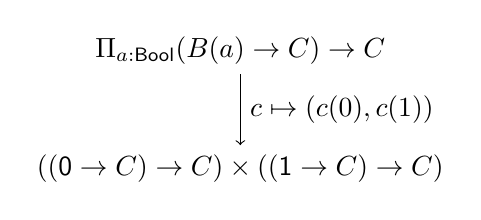
\begin{tikzpicture}
\node (N0) at (0,12) {$\prd{a:\Bool} (B(a) \to C) \to C$};
\node (N1) at (0,10.5) {$((\zero \to C) \to C) \times ((\one \to C) \to C)$};
\draw[->] (N0) -- node[right]{$c \mapsto (c(0), c(1))$} (N1);
\end{tikzpicture}
\end{center}
The type $\zero \to C$ is contractible with center $(\lambda b:\zero) \abort(C,b)$. We thus have an equivalence
\begin{center}
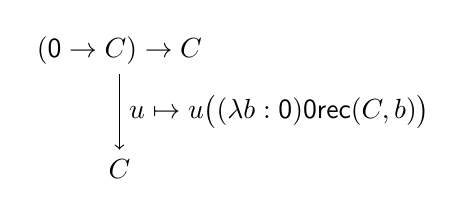
\begin{tikzpicture}
\node (N0) at (0,12) {$(\zero \to C) \to C$};
\node (N1) at (0,10.5) {$C$};
\draw[->] (N0) -- node[right]{$u \mapsto u\big((\lambda b:\zero) \abort(C,b)\big)$} (N1);
\end{tikzpicture}
\end{center}
Since the map $x \mapsto (\lambda \_:\one)x$ is an equivalence from $C$ to $\one \to C$, we have an equivalence
\begin{center}
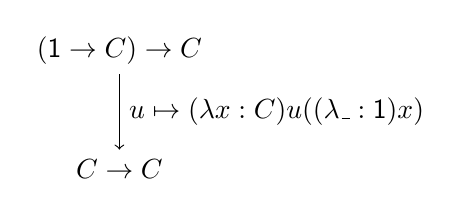
\begin{tikzpicture}
\node (N0) at (0,12) {$(\one \to C) \to C$};
\node (N1) at (0,10.5) {$C \to C$};
\draw[->] (N0) -- node[right]{$u \mapsto (\lambda x:C) u((\lambda \_:\one)x)$} (N1);
\end{tikzpicture}
\end{center}
Putting this all together, we see that the map 
\[ (C,c) \mapsto \Big(C,c\big(0,(\lambda b:\zero) \abort(C,b)\big),(\lambda x:C) c(1, (\lambda \_:\one)x)\Big)\] 
is an equivalence from $\WAlg(A,B)$ to $\NatAlg$.
\end{proof}

\begin{lemma}
For any $P$-algebra $\X : \WAlg(A,B)$ there is an equivalence
\[ \WFibAlgToNatFibAlg : \WFibAlg \; \X \to \NatFibAlg \; (\WAlgToNatAlg(\X)) \]
\end{lemma}
\begin{proof}
Let $(C,c)$ be a $P$-algebra and fix $E : C \to \U$. We have an equivalence
\begin{center}
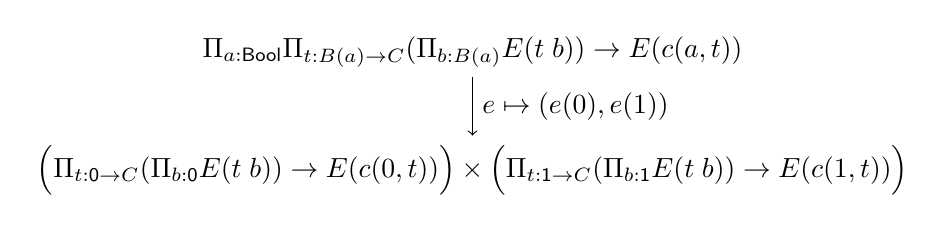
\begin{tikzpicture}
\node (N0) at (0,12) {$\prd{a:\Bool}\prd{t:B(a)\to C} (\prd{b:B(a)} E(t\;b)) \to E(c(a,t))$};
\node (N1) at (0,10.5) {$\Big(\prd{t:\zero\to C} (\prd{b:\zero} E(t\;b)) \to E(c(0,t))\Big) \times \Big(\prd{t:\one\to C} (\prd{b:\one} E(t\;b)) \to E(c(1,t))\Big)$};
\draw[->] (N0) -- node[right]{$e \mapsto (e(0), e(1))$} (N1);
\end{tikzpicture}
\end{center}
The type $\zero \to C$ is contractible with center $(\lambda b:\zero) \abort(C,b)$. Likewise, the type $\prd{b:\zero} E(\abort(C,b))$ is contractible with center 
$(\lambda b:\zero) \abort\big(E(\abort(C,b)),b\big)$. We thus have equivalences
\begin{center}
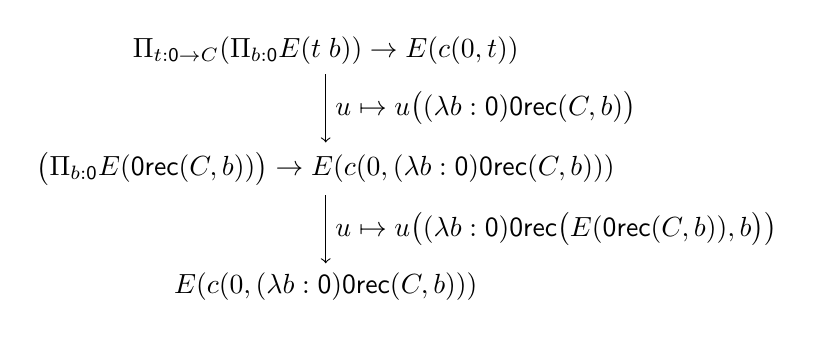
\begin{tikzpicture}
\node (N0) at (0,12) {$\prd{t:\zero\to C} (\prd{b:\zero} E(t\;b)) \to E(c(0,t))$};
\node (N1) at (0,10.5) {$\big(\prd{b:\zero} E(\abort(C,b))\big) \to E(c(0,(\lambda b:\zero) \abort(C,b)))$};
\node (N2) at (0,9) {$E(c(0,(\lambda b:\zero) \abort(C,b)))$};
\draw[->] (N0) -- node[right]{$u \mapsto u\big((\lambda b:\zero) \abort(C,b)\big)$} (N1);
\draw[->] (N1) -- node[right]{$u \mapsto u\big((\lambda b:\zero) \abort\big(E(\abort(C,b)),b\big)\big)$} (N2);
\end{tikzpicture}
\end{center}
The map $x \mapsto (\lambda \_:\one)x$ is an equivalence from $C$ to $\one \to C$. Likewise, for any $x:C$ the map $y \mapsto (\lambda \_:\one)y$  is an equivalence from $E(x)$ to $\one \to E(x)$. Thus, we have equivalences
\begin{center}
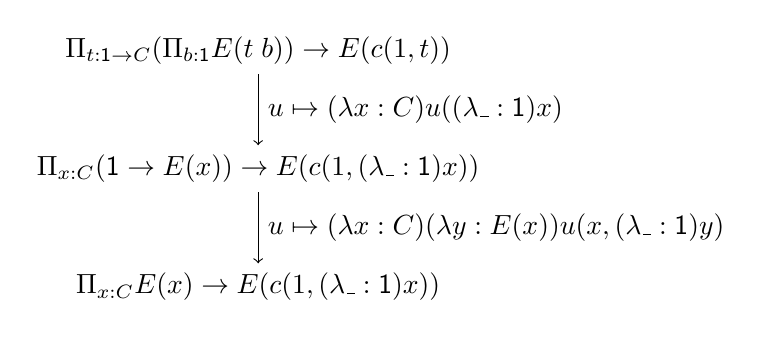
\begin{tikzpicture}
\node (N0) at (0,12) {$\prd{t:\one\to C} (\prd{b:\one} E(t\;b)) \to E(c(1,t))$};
\node (N1) at (0,10.5) {$\prd{x:C} (\one \to E(x)) \to E(c(1,(\lambda \_:\one)x))$};
\node (N2) at (0,9) {$\prd{x:C} E(x) \to E(c(1,(\lambda \_:\one)x))$};
\draw[->] (N0) -- node[right]{$u \mapsto (\lambda x:C) u((\lambda \_:\one)x)$} (N1);
\draw[->] (N1) -- node[right]{$u \mapsto (\lambda x:C) (\lambda y:E(x)) u(x,(\lambda \_:\one)y)$} (N2);
\end{tikzpicture}
\end{center}
Putting this all together, we see that the map 
\begin{align*}
& (E,e) \mapsto \Big(E,e\big(0,(\lambda b:\zero) \abort(C,b), (\lambda b:\zero) \abort\big(E(\abort(C,b)),b\big)\big),\\ & \;\;\;\;\;\;\;\;\;\;\;\;\;\;\;\;\;\;\;\;\;\;\;\; (\lambda x:C) (\lambda y:E(x)) e(1, (\lambda \_:\one)x), (\lambda \_:\one)y\Big)
\end{align*}
is an equivalence from $\WFibAlg \; (C,c)$ to $\NatFibAlg \; (\WAlgToNatAlg \; (C,c))$.
\end{proof}

\begin{lemma}
For any $P$-algebra $\X : \WAlg(A,B)$ and fibered $P$-algebra $\Y : \WFibAlg \; \X$ over $\X$ we have
\[ \WFibHom \; \Y \;\; \simeq \;\; \NatFibHom \; \big(\WFibAlgToNatFibAlg(\Y)\big) \]
\end{lemma}
\begin{proof}
Let $(C,c)$ be a $P$-algebra and $(E,e)$ be a fibered $P$-algebra over $(C,c)$. Fix a function $f : (\Pi x:C) E(x)$. We have an equivalence
\begin{center}
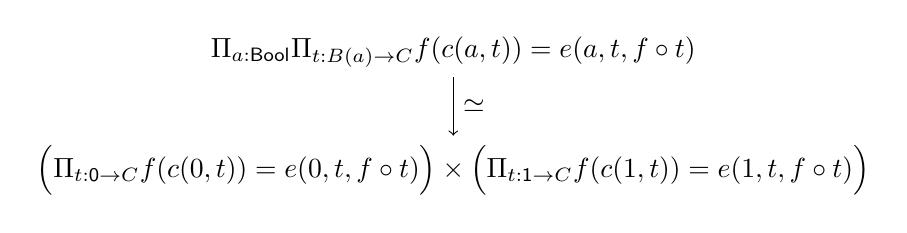
\begin{tikzpicture}
\node (N0) at (0,12) {$\prd{a:\Bool}\prd{t:B(a)\to C} f(c(a,t)) = e(a,t,f \circ t)$};
\node (N1) at (0,10.5) {$\Big(\prd{t:\zero\to C} f(c(0,t)) = e(0,t,f \circ t)\Big) \times \Big(\prd{t:\one\to C} f(c(1,t)) = e(1,t,f \circ t)\Big)$};
\draw[->] (N0) -- node[right]{$\simeq$} (N1);
\end{tikzpicture}
\end{center}
The type $\zero \to C$ is contractible with center $(\lambda b:\zero) \abort(C,b)$. Furthermore, since all functions out of $\zero$ having the same codomain are equal, we have
\[f \circ (\lambda b:\zero) \abort(C,b) = (\lambda b:\zero) \abort(E(\abort(C,b)), b)\]
This implies the following equivalences:
\begin{center}
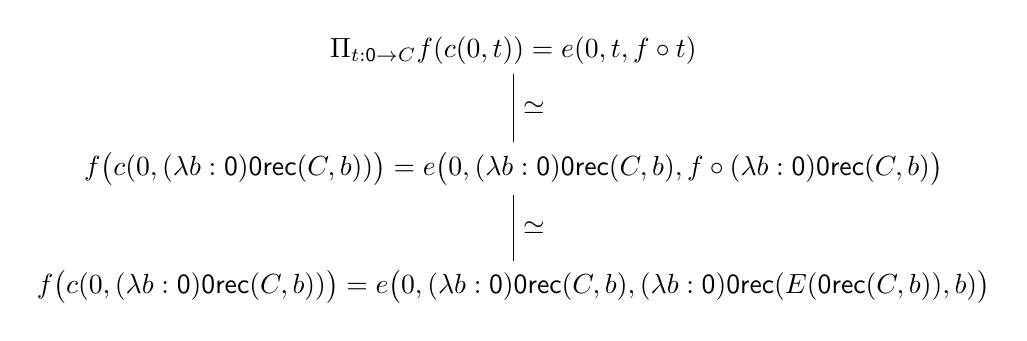
\begin{tikzpicture}
\node (N0) at (0,12) {$\prd{t:\zero\to C} f(c(0,t)) = e(0,t,f \circ t)$};
\node (N1) at (0,10.5) {$f\big(c(0,(\lambda b:\zero) \abort(C,b))\big) = e\big(0,(\lambda b:\zero) \abort(C,b), f \circ (\lambda b:\zero) \abort(C,b)\big)$};
\node (N2) at (0,9) {$f\big(c(0,(\lambda b:\zero) \abort(C,b))\big) = e\big(0,(\lambda b:\zero) \abort(C,b),(\lambda b:\zero) \abort(E(\abort(C,b)), b)\big)$};
\draw[-] (N0) -- node[right]{$\simeq$} (N1);
\draw[-] (N1) -- node[right]{$\simeq$} (N2);
\end{tikzpicture}
\end{center}
The map $x \mapsto (\lambda \_:\one)x$ is an equivalence from $C$ to $\one \to C$.  Thus, we have an equivalence
\begin{center}
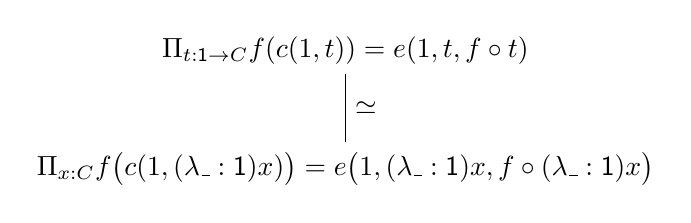
\begin{tikzpicture}
\node (N0) at (0,12) {$\prd{t:\one\to C} f(c(1,t)) = e(1,t,f \circ t)$};
\node (N1) at (0,10.5) {$\prd{x:C} f\big(c(1,(\lambda \_:\one)x)\big) = e\big(1,(\lambda \_:\one)x, f \circ (\lambda \_:\one)x\big)$};
\draw[-] (N0) -- node[right]{$\simeq$} (N1);
\end{tikzpicture}
\end{center}
This finishes the proof.
\end{proof}

\begin{corollary}
For any $P$-algebras $\X,\Y : \WAlg(A,B)$ we have
\[ \WHom \; \X \; \Y \;\; \simeq \;\; \NatHom \; \big(\WAlgToNatAlg(\X)\big) \; \big(\WAlgToNatAlg(\Y)\big) \]
\end{corollary}

\begin{corollary}
For any $\nat$-algebra $\X : \NatAlg$ we have
\begin{alignat*}{4}
& \IsNatHInit(\X) \;\; & \simeq \;\; & \IsWHInit(\WAlgToNatAlg^{-1}(\X)) \\
& \IsNatHProj(\X) \;\; & \simeq \;\; & \IsWHProj(\WAlgToNatAlg^{-1}(\X))
\end{alignat*}
\end{corollary}

\begin{theorem}\label{lem:WMainInternal}
For a $\nat$-algebra $\X : \NatAlg$, we have
\[ \IsNatHProj \; \X \;\;\; \leftrightarrow \;\;\; \IsNatHInit \; \X \]
Moreover, both types are mere propositions; hence in particular we have
\[ \IsNatHProj \; \X \;\;\; \simeq \;\;\; \IsNatHInit \; \X \]
\end{theorem}

\begin{corollary}\label{lem:NatInitInt}
The $\nat$ algebra $(\nat,\z,\suc(-)) : \NatAlg$ is homotopy-initial.
\end{corollary}

\section{Acknowledgements}

We would like to thank Vladimir Voevodsky and Michael Warren for helpful discussions
on the subject of this paper. In particular, Vladimir Voevodsky suggested a simplification of the 
proof that the rules for homotopical W-types imply h-initiality.

Steve Awodey gratefully acknowledges the support of the National Science Foundation, Grant DMS-1001191
 and the Air Force OSR, Grant 11NL035.
Nicola Gambino is grateful for the support of the Institute for Advanced Study, where
he worked on this project. This work was supported by the National Science Foundation 
under agreement No.\ DMS-0635607. Any opinions, findings and conclusions or recommendations
expressed in this material are those of the authors and do not necessarily reflect the views of
the National Science Foundation.
Kristina Sojakova is grateful for the support of CyLab at Carnegie
Mellon under grants DAAD19-02-1-0389 and W911NF-09-1-0273 from the Army
Research Office.



\appendix

\section{Type-theoretic rules}


\begin{table}[ht]
\fbox{ 
\begin{minipage}{12cm}
\medskip
\begin{itemize}
\item Formation rule
\[
\begin{prooftree}
x \co A \vdash B(x) \co \type
\justifies
(\Pi x \co A) B(x) \co \type
\end{prooftree}
\]
\item Introduction rule
\[
\begin{prooftree}
x \co A \vdash b(x) \co B(x) 
\justifies
(\lambda x \co A)b(x) \co (\Pi x : A) B(x)
\end{prooftree}
\]
\item Elimination rule
\[
\begin{prooftree}
f \co (\Pi x : A) B(x) \quad
a \co A 
\justifies
\app(f, a) \co B(a)
\end{prooftree}
\]
\item $\beta$-rule
\[
\begin{prooftree}
x \co A \vdash b(x) \co B(x) 
\justifies
\app( (\lambda x : A) b(x), a) \equiv b(a) \co B(a)
\end{prooftree}
\]
\item $\eta$-rule
\[
\begin{prooftree}
f \co (\Pi x :A) B(x) 
\justifies
f \equiv (\lambda x : A) \app(f, x) \co (\Pi x \co A) B(x)
\end{prooftree}
\]
 \end{itemize} \medskip
\end{minipage}}
\medskip
\caption{Rules for $\Pi$-types.}
\label{tab:pi}
\end{table}


\begin{table}[ht]
\fbox{ 
\begin{minipage}{12cm}
\medskip
\begin{itemize}
\item Formation rule
\[
\begin{prooftree}
x \co A \vdash B(x) \co \type
\justifies
(\Sigma x \co A) B(x) \co \type
\end{prooftree}
\]
\item Introduction rule
\[
\begin{prooftree}
a \co A \qquad 
b(a) \co B(a) 
\justifies
\pair(a,b) \co (\Sigma x : A) B(x)
\end{prooftree}
\]
\item $\Sigma$-elimination rule.
\[
\begin{prooftree}
\begin{array}{l} 
u : (\Sigma x : A) B(x) \vdash E(u) :  \type \\
 x :  A, y \co B(x) \vdash  e(x,y) :  E(\pair(x,y))  
 \end{array}
\justifies
u :  (\Sigma x :A)B(x) \vdash  \mysplit(u,e) :  E(u)
\end{prooftree}
\]
\item $\Sigma$-computation rule.
\[
\begin{prooftree}
\begin{array}{l} 
u : (\Sigma x : A) B(x) \vdash E(u) :  \type \\
 x :  A, y \co B(x) \vdash  e(x,y) :  E(\pair(x,y))  
 \end{array}
 \justifies
x :  A, y \co B(x) \vdash \mysplit(\pair(x,y),e) \equiv e(x,y) :  E(\pair(x,y)) \, .
\end{prooftree}
\]
\end{itemize} \medskip
\end{minipage}}
\medskip
\caption{Rules for $\Sigma$-types.}
\label{tab:sigma}
\end{table}




\begin{table}[ht]
\fbox{ 
\begin{minipage}{12cm}
\medskip
\begin{itemize}
\item $\Id$-formation rule.
\[
\begin{prooftree}
A :  \type \quad 
a :  A  \quad
b :  A 
\justifies
 \id{A}(a,b) :  \type
 \end{prooftree}
\]
\item $\Id$-introduction rule.
\[
\begin{prooftree}
a :  A 
\justifies
 \refl(a) :  \id{A}(a,a)
 \end{prooftree} 
\]
\item $\Id$-elimination rule.
\[
\begin{prooftree}
\begin{array}{l} 
x, y :  A, u :  \id{A}(x,y) \vdash E(x,y,u) :  \type \\
 x :  A \vdash  e(x) :  E(x,x,\refl(x))  
 \end{array}
\justifies
x, y :  A, u :  \id{A}(x,y) \vdash  \idrec(x,y,u,e) :  E(x,y,u)
\end{prooftree}
\]
\item $\Id$-computation rule.
\[
\begin{prooftree}
\begin{array}{l} 
x, y :  A, u :  \id{A}(x,y) \vdash E(x,y,u) :  \type \\
 x :  A \vdash  e(x) :  E(x,x,\refl(x)) 
 \end{array}
 \justifies
x :  A \vdash \idrec(x,x,\refl(x), e) = e(x) :  E(x, x, \refl(x)) \, .
\end{prooftree}
\]
\end{itemize} \medskip
\end{minipage}}
\medskip
\caption{Rules for $\Id$-types.}
\label{tab:id}
\end{table}




\begin{table}[ht]
\fbox{ 
\begin{minipage}{12cm}
\medskip
\begin{itemize}
\item Formation rule. \smallskip

\[
 \Bool : \UU \, .
 \]  \medskip
\item Introduction rules. \smallskip

\[
0 : \Bool \, ,  \qquad  1 : \Bool \, .
\]  
\item Elimination rule.\medskip

\[
\begin{prooftree}
x:\Bool \vdash E(x) : \UU \qquad
e_0 : E(0) \qquad
e_1 : E(1) \qquad
\justifies
x \co \Bool \vdash \boolind(x, e_0, e_1) : E(x) 
\end{prooftree}
\] \bigskip
\item Computation rules. \smallskip

\begin{equation*}
\begin{prooftree}
x:\Bool \vdash E(x) : \UU \qquad
e_0 : E(0) \qquad
e_1 : E(1)
\justifies
  \boolind(0, e_0, e_1)  \deq  e_0 \co E(0) \, , \\
\end{prooftree}
 \end{equation*}  
 \bigskip
 \begin{equation*}
\begin{prooftree}
x:\Bool \vdash E(x) : \UU \qquad
e_0 : E(0) \qquad
e_1 : E(1)
\justifies
 \boolind(1,e_0,e_1)  \deq e_1 \co E(1) \, .
\end{prooftree}
 \end{equation*}  
\end{itemize}
\medskip
\end{minipage}}
\medskip
\caption{Deduction rules for the type $\Bool$.}
\label{tab:bool} 
\end{table}



\bibliographystyle{plain}

\bibliography{references}
                        


\end{document}